\begin{appendices}
    
\section{Cadence global statistics}
\label{sec:globalstat}

%\begin{table}
%\begin{center}
\begin{longtable}{l|ccccccc}
    \caption{Global filter allocation of all cadences studied in this note.}\label{tab:global_cadence_stats} \\
    \hline
    \hline    
  name & \multicolumn{7}{c}{\# visits} \\
       & $u$ & $g$ & $r$ & $i$ & $z$ & $y$ & Total \\

  \hline
  \hline
  \multicolumn{8}{c}{Cadences simulated for the White paper call}\\
  \hline      
      baseline 2018a &  177538 &  234144 &  515172 &  514481 &  486208 &  445157 &  2372700 \\ 
                     &    7.5 \% &    9.9 \% &   21.7 \% &   21.7 \% &   20.5 \% &   18.8 \% & \\
\hline
         kraken 2035 &  176828 &  237799 &  522679 &  520282 &  497539 &  454450 &  2409577 \\ 
                     &    7.3 \% &    9.9 \% &   21.7 \% &   21.6 \% &   20.6 \% &   18.9 \% & \\
\hline         
         kraken 2042 &  197391 &  258590 &  571414 &  567785 &  529266 &  484923 &  2609369 \\ 
                     &    7.6 \% &    9.9 \% &   21.9 \% &   21.8 \% &   20.3 \% &   18.6 \% & \\
\hline
         kraken 2036 &  150652 &  200360 &  441677 &  439015 &  443328 &  392881 &  2067913 \\ 
                     &    7.3 \% &    9.7 \% &   21.4 \% &   21.2 \% &   21.4 \% &   19.0 \% & \\
\hline
         kraken 2044 &  179340 &  230010 &  520373 &  519688 &  509678 &  492524 &  2451613 \\ 
                     &    7.3 \% &    9.4 \% &   21.2 \% &   21.2 \% &   20.8 \% &   20.1 \% & \\
\hline
         kraken 2026 &  182465 &  241422 &  532326 &  529190 &  496037 &  456948 &  2438388 \\ 
                     &    7.5 \% &    9.9 \% &   21.8 \% &   21.7 \% &   20.3 \% &   18.7 \% & \\
\hline
       colossus 2665 &  182959 &  238121 &  527822 &  524508 &  494317 &  458122 &  2425849 \\ 
                     &    7.5 \% &    9.8 \% &   21.8 \% &   21.6 \% &   20.4 \% &   18.9 \% & \\
\hline
       colossus 2667 &  185815 &  242738 &  534218 &  533143 &  517513 &  479169 &  2492596 \\ 
                     &    7.5 \% &    9.7 \% &   21.4 \% &   21.4 \% &   20.8 \% &   19.2 \% & \\
\hline
       colossus 2664 &  179185 &  237797 &  533279 &  530020 &  500969 &  459024 &  2440274 \\ 
                     &    7.3 \% &    9.7 \% &   21.9 \% &   21.7 \% &   20.5 \% &   18.8 \% & \\
\hline
         pontus 2502 &  128795 &  186756 &  421971 &  426707 &  370248 &  499345 &  2033822 \\ 
                     &    6.3 \% &    9.2 \% &   20.7 \% &   21.0 \% &   18.2 \% &   24.6 \% & \\
\hline
         pontus 2002 &  176036 &  228309 &  519417 &  518145 &  494484 &  489085 &  2425476 \\ 
                     &    7.3 \% &    9.4 \% &   21.4 \% &   21.4 \% &   20.4 \% &   20.2 \% & \\
\hline
         pontus 2489 &  242197 &  334560 &  740905 &  735996 &  707598 &  645786 &  3407042 \\ 
                     &    7.1 \% &    9.8 \% &   21.7 \% &   21.6 \% &   20.8 \% &   19.0 \% & \\
\hline
         mothra 2049 &  174249 &  221754 &  510555 &  507512 &  547373 &  487791 &  2449234 \\ 
                     &    7.1 \% &    9.1 \% &   20.8 \% &   20.7 \% &   22.3 \% &   19.9 \% & \\
\hline
         mothra 2045 &  124930 &  162090 &  358798 &  348781 &  431698 &  373624 &  1799921 \\ 
                     &    6.9 \% &    9.0 \% &   19.9 \% &   19.4 \% &   24.0 \% &   20.8 \% & \\
\hline
          nexus 2097 &  169168 &  220984 &  508305 &  508811 &  532379 &  502140 &  2441787 \\ 
                     &    6.9 \% &    9.1 \% &   20.8 \% &   20.8 \% &   21.8 \% &   20.6 \% & \\
\hline
\hline
\multicolumn{8}{c}{Pre-white paper call cadences}\\
\hline
         minion 1016 &  181479 &  246667 &  538936 &  541688 &  493206 &  446306 &  2448282 \\ 
                     &    7.4 \% &   10.1 \% &   22.0 \% &   22.1 \% &   20.1 \% &   18.2 \% & \\
\hline
feature rolling half mask &  161705 &  248253 &  498985 &  500143 &  468829 &  407239 &  2285154 \\ 
                     &    7.1 \% &   10.9 \% &   21.8 \% &   21.9 \% &   20.5 \% &   17.8 \% & \\
\hline
 feature rolling 2/3 &  168475 &  249395 &  485866 &  487889 &  458198 &  392546 &  2242369 \\ 
                     &    7.5 \% &   11.1 \% &   21.7 \% &   21.8 \% &   20.4 \% &   17.5 \% & \\
\hline
     blobs mix zmask &  136179 &  210526 &  466483 &  490187 &  460636 &  422157 &  2186168 \\ 
                     &    6.2 \% &    9.6 \% &   21.3 \% &   22.4 \% &   21.1 \% &   19.3 \% & \\
\hline
          blobs same &  136248 &  210601 &  491842 &  499587 &  464083 &  425724 &  2228085 \\ 
                     &    6.1 \% &    9.5 \% &   22.1 \% &   22.4 \% &   20.8 \% &   19.1 \% & \\
\hline
    blobs same zmask &  136581 &  210621 &  494712 &  502383 &  466958 &  428173 &  2239428 \\ 
                     &    6.1 \% &    9.4 \% &   22.1 \% &   22.4 \% &   20.9 \% &   19.1 \% & \\
\hline
         rolling mix &  136421 &  182049 &  494744 &  491103 &  465629 &  433587 &  2203533 \\ 
                     &    6.2 \% &    8.3 \% &   22.5 \% &   22.3 \% &   21.1 \% &   19.7 \% & \\
\hline
    feature baseline &  159252 &  245015 &  503803 &  506598 &  474436 &  415687 &  2304791 \\ 
                     &    6.9 \% &   10.6 \% &   21.9 \% &   22.0 \% &   20.6 \% &   18.0 \% & \\
\hline
\hline
\multicolumn{8}{c}{\altsched~family}\\
\hline
       \altsched~wide &  175870 &  229198 &  585108 &  386768 &  543465 &  149779 &  2070188 \\ 
                     &    8.5 \% &   11.1 \% &   28.3 \% &   18.7 \% &   26.3 \% &    7.2 \% & \\
\hline
       \altsched~wide &  174191 &  224852 &  583361 &  390035 &  542420 &  164683 &  2079542 \\ 
                     &    8.4 \% &   10.8 \% &   28.1 \% &   18.8 \% &   26.1 \% &    7.9 \% & \\
       \hline
    \altsched~rolling &  158792 &  203909 &  567306 &  376261 &  556285 &  186852 &  2049405 \\ 
                     &    7.7 \% &    9.9 \% &   27.7 \% &   18.4 \% &   27.1 \% &    9.1 \% & \\
\hline
            \altsched &  170952 &  221660 &  570519 &  376786 &  529925 &  177866 &  2047708 \\ 
                     &    8.3 \% &   10.8 \% &   27.9 \% &   18.4 \% &   25.9 \% &    8.7 \% & \\
\hline
       \altsched (GW) &  170952 &  221660 &  570519 &  376786 &  529925 &  177866 &  2047708 \\ 
                     &    8.3 \% &   10.8 \% &   27.9 \% &   18.4 \% &   25.9 \% &    8.7 \% & \\
\hline
 \altsched + twilight &  170952 &  481678 &  570519 &  376786 &  529925 &  177866 &  2307726 \\ 
                     &    7.4 \% &   20.9 \% &   24.7 \% &   16.3 \% &   23.0 \% &    7.7 \% & \\

\hline
\hline
\multicolumn{8}{c}{SLAIR experimental cadences}\\
\hline
   tight\_mask\_simple &   95701 &  171752 &  521284 &  524906 &  474108 &  352726 &  2140477 \\ 
                     &    4.5 \% &    8.0 \% &   24.4 \% &   24.5 \% &   22.1 \% &   16.5 \% & \\
\hline
          tight\_mask &  123055 &  198521 &  544609 &  547906 &  494370 &  222879 &  2131340 \\ 
                     &    5.8 \% &    9.3 \% &   25.6 \% &   25.7 \% &   23.2 \% &   10.5 \% & \\
\hline
            tms\_roll &  131805 &  188634 &  451325 &  453669 &  415830 &  468191 &  2109454 \\ 
                     &    6.2 \% &    8.9 \% &   21.4 \% &   21.5 \% &   19.7 \% &   22.2 \% & \\
\hline
           tms\_drive &  145891 &  204920 &  462039 &  465567 &  428663 &  388628 &  2095708 \\ 
                     &    7.0 \% &    9.8 \% &   22.0 \% &   22.2 \% &   20.5 \% &   18.5 \% & \\
\hline
     rolling (slair) &  136116 &  207232 &  513500 &  512608 &  462963 &  432323 &  2264742 \\ 
                     &    6.0 \% &    9.2 \% &   22.7 \% &   22.6 \% &   20.4 \% &   19.1 \% & \\
\hline
      rolling mix 75 &  138131 &  180878 &  486583 &  480726 &  457204 &  426237 &  2169759 \\ 
                     &    6.4 \% &    8.3 \% &   22.4 \% &   22.2 \% &   21.1 \% &   19.6 \% & \\
\hline
         cadence mix &  152016 &  224174 &  467748 &  473170 &  436180 &  408400 &  2161688 \\ 
                     &    7.0 \% &   10.4 \% &   21.6 \% &   21.9 \% &   20.2 \% &   18.9 \% & \\
         \hline
\end{longtable}
%\end{center}
  %\end{table}
\begin{longtable}{l|l|cccc}
  \caption{Specific SN cadence statistics\label{tab:sn_specific_cadence_stats}}        \\
  \hline
  \hline    
  name & & \multicolumn{4}{c}{ bands } \\
       & & $g$ & $r$ & $i$ & $z$  \\

  \hline
  \hline
  \multicolumn{6}{c}{Cadences simulated for the White paper call}\\
  \hline      
  baseline 2018a & \# visits                   &   52  & 117  & 117  & 105   \\
                 & mean $\delta t$ between obs &   23  &  12  &  12  &  14   \\
                 & 15+ day gaps                &   0.6 & 0.3  & 0.3  &  0.4  \\
                 & median season length               & \multicolumn{4}{c}{145} \\
  \hline
  kraken 2035    & \# visits                   &   52 &  115 &  115 &  104 \\
                 & mean $\delta t$ between obs &   24 &   12 &   12 &   14 \\
                 & 15+ day gaps                &  0.6 &  0.4 &  0.3 &  0.4 \\
                 & median season length               & \multicolumn{4}{c}{168}   \\
  \hline

  kraken 2042    & \# visits                   &   53 &  120 &  120 &  107 \\
                 & mean $\delta t$ between obs &  25  &   12 &   12 &   14 \\
                 & 15+ day gaps                &  0.6 &  0.3 &  0.3 &  0.4 \\
                 & median season length               & \multicolumn{4}{c}{174}   \\
  \hline

  kraken 2036    & \# visits                   &  43  &   95 &   95 &   91 \\
                 & mean $\delta t$ between obs &  17  &    9 &    9 &   10 \\
                 & 15+ day gaps                &  0.4 &   0.2&  0.2 &  0.3 \\
                 & median season length               & \multicolumn{4}{c}{157}   \\
  \hline

  kraken 2044    & \# visits                   &  68  &  154 &  153 & 147  \\
                 & mean $\delta t$ between obs &  19  &    9 &   10 &  11  \\
                 & 15+ day gaps                & 0.5  &  0.3 &  0.2 & 0.3  \\
                 & median season length               & \multicolumn{4}{c}{173}   \\
  \hline

  kraken 2026    & \# visits                   &  55  & 122  & 121  & 108  \\
                 & mean $\delta t$ between obs &  23  &  12  &  12  &  14  \\
                 & 15+ day gaps                & 0.6  & 0.3  & 0.3  & 0.4  \\
                 & median season length               & \multicolumn{4}{c}{170}   \\
  \hline

  colossus 2665  & \# visits                   &  53  & 117  & 116  & 104  \\
                 & mean $\delta t$ between obs &  23  &  12  &  12  &  14  \\
                 & 15+ day gaps                & 0.6  & 0.3  & 0.3  & 0.4  \\
                 & median season length               & \multicolumn{4}{c}{168}   \\
  \hline

  colossus 2667  & \# visits                   &  76  & 173  &  172 &  163 \\
                 & mean $\delta t$ between obs &  18  &   9  &    9 &   11 \\
                 & 15+ day gaps                &  0.5 & 0.3  & 0.2  &  0.3 \\
                 & median season length               & \multicolumn{4}{c}{187}   \\
  \hline

  colossus 2664  & \# visits                   &  53  & 120  & 119  & 106  \\
                 & mean $\delta t$ between obs &  23  &  12  &  12  &  14  \\
                 & 15+ day gaps                & 0.6  & 0.3  & 0.3  & 0.4  \\
                 & median season length               & \multicolumn{4}{c}{165}   \\
  \hline
  
  pontus 2502    & \# visits                   &  38  &  85  &  87  &  72  \\
                 & mean $\delta t$ between obs &  23  &  14  &  14  &  15  \\
                 & 15+ day gaps                & 0.6  & 0.4  & 0.3  & 0.4  \\
                 & median season length               & \multicolumn{4}{c}{179}   \\
  \hline

  pontus 2002    & \# visits                   &  44  &  99  &  98  &  88  \\
                 & mean $\delta t$ between obs &  25  &  14  &  14  &  15  \\
                 & 15+ day gaps                & 0.6  & 0.4  & 0.3  & 0.4  \\
                 & median season length               & \multicolumn{4}{c}{158}   \\
  \hline

  pontus 2489    & \# visits                   &  72  & 163  & 160  &  148 \\
                 & mean $\delta t$ between obs &  19  &   9  &   9  &   11 \\
                 & 15+ day gaps                & 0.5  & 0.2  & 0.2  &  0.3 \\
                 & median season length               & \multicolumn{4}{c}{180}   \\
  \hline

  mothra 2049    & \# visits                   &   37 &  85  &  85  &  88  \\
                 & mean $\delta t$ between obs &   16 &   8  &   8  &   9  \\
                 & 15+ day gaps                &  0.4 & 0.2  & 0.2  & 0.3  \\
                 & median season length               & \multicolumn{4}{c}{172}   \\
  \hline

  mothra 2045    & \# visits                   &   31 &  64  &  61  &  85  \\
                 & mean $\delta t$ between obs &   17 &   9  &  11  &   9  \\
                 & 15+ day gaps                &  0.4 & 0.2  & 0.2  & 0.3  \\
                 & median season length               & \multicolumn{4}{c}{157}   \\
  \hline

  nexus 2097     & \# visits                   &  37  &  83  &  84  &  85  \\
                 & mean $\delta t$ between obs &  17  &  10  &  10  &   9  \\
                 & 15+ day gaps                & 0.4  & 0.3  & 0.2  & 0.3  \\
                 & median season length               & \multicolumn{4}{c}{162}   \\
  \hline
  \hline
  \multicolumn{6}{c}{Pre-white paper call cadences}\\
  \hline

  minion 1016    & \# visits                   &   49 & 101  &  96  & 103  \\
                 & mean $\delta t$ between obs &   29 &  16  &  17  &  18  \\
                 & 15+ day gaps                &  0.7 & 0.4  & 0.4  & 0.4  \\
                 & median season length               & \multicolumn{4}{c}{213}   \\
  \hline

  feature rolling half mask & \# visits        &  29  &  63  &  61  &  53  \\
                 & mean $\delta t$ between obs &  17  &  13  &  13  &  14  \\
                 & 15+ day gaps                & 0.5  & 0.3  & 0.3  & 0.4  \\
                 & median season length               & \multicolumn{4}{c}{133}   \\
  \hline

  feature rolling 2/3       & \# visits        &  25  &  52  &  52  & 45   \\
                 & mean $\delta t$ between obs &  14  &  11  &  11  & 12   \\
                 & 15+ day gaps                & 0.4  & 0.2  & 0.2  & 0.3  \\
                 & median season length               & \multicolumn{4}{c}{137}   \\
  \hline

 blobs mix zmask & \# visits                   &  72  & 166  &  168 & 118  \\
                 & mean $\delta t$ between obs &  20  &  11  &   11 &  16  \\
                 & 15+ day gaps                & 0.6  & 0.3  &  0.3 & 0.4  \\
                 & median season length               & \multicolumn{4}{c}{187}   \\
  \hline
  
 blobs same      & \# visits                   &  35  &  90  &  96  & 122  \\
                 & mean $\delta t$ between obs &  33  &  20  &  18  &  15  \\
                 & 15+ day gaps                & 0.8  & 0.6  & 0.5  & 0.4  \\
                 & median season length               & \multicolumn{4}{c}{186}   \\
  \hline

 blobs same zmask& \# visits                   &  35  & 90   &  96  & 120  \\
                 & mean $\delta t$ between obs &  33  & 20   &  18  &  15  \\
                 & 15+ day gaps                & 0.8  &0.6   & 0.5  & 0.4  \\
                 & median season length               & \multicolumn{4}{c}{188}   \\
  \hline
  
  rolling mix    & \# visits                   &  67  & 178  & 178  & 124  \\
                 & mean $\delta t$ between obs &  14  &   8  &   8  &  12  \\
                 & 15+ day gaps                & 0.4  & 0.2  & 0.2  & 0.3  \\
                 & median season length               & \multicolumn{4}{c}{179}   \\
  \hline

feature baseline & \# visits                   &  30  &  66  &  67  &  58  \\
                 & mean $\delta t$ between obs &  27  &  20  &  20  &  22  \\
                 & 15+ day gaps                & 0.7  & 0.5  & 0.5  & 0.6  \\
                 & median season length               & \multicolumn{4}{c}{146}   \\
  \hline
  \hline
  \multicolumn{6}{c}{Altsched family}\\
  \hline
 altsched wide   & \# visits                   &  78  & 201  & 133  & 169  \\
                 & mean $\delta t$ between obs &  16  &   7  &   9  &   8  \\
                 & 15+ day gaps                & 0.4  & 0.1  & 0.2  & 0.1  \\
                 & median season length               & \multicolumn{4}{c}{140}   \\
  \hline

 altsched rolling& \# visits                   &   93 &  258 & 172  & 230  \\
                 & mean $\delta t$ between obs &    8 &    3 &   4  &   3  \\
                 & 15+ day gaps                &  0.2 & $<0.05$& $<0.05$ &  $<0.05$\\
                 & median season length               & \multicolumn{4}{c}{151}   \\
  \hline

  altsched       & \# visits                   & 102  & 261  & 175  & 222  \\
                 & mean $\delta t$ between obs &  14  &   6  &   8  &   7  \\
                 & 15+ day gaps                & 0.3  &$<0.1$&$<0.1$&  0.1 \\
                 & median season length               & \multicolumn{4}{c}{150}   \\
  \hline
  \hline
  \multicolumn{6}{c}{SLAIR experimental cadences}\\
  \hline

tight mask simple& \# visits                   &  50  & 153  & 153  & 111  \\
                 & mean $\delta t$ between obs &  16  &  10  &  10  &  12  \\
                 & 15+ day gaps                & 0.4  & 0.2  & 0.2  & 0.3  \\
                 & median season length               & \multicolumn{4}{c}{154}   \\
  \hline

tight mask       & \# visits                   &  60  & 164  & 163  & 117  \\
                 & mean $\delta t$ between obs &  15  &   9  &   9  &  12  \\
                 & 15+ day gaps                & 0.4  & 0.2  & 0.2  & 0.3  \\
                 & median season length               & \multicolumn{4}{c}{155}   \\
  \hline

tms roll         & \# visits                   &  60  & 159  & 158  &  123 \\
                 & mean $\delta t$ between obs &  12  &   7  &   7  &    9 \\
                 & 15+ day gaps                & 0.3  & 0.1  & 0.1  &  0.2 \\
                 & median season length               & \multicolumn{4}{c}{154}   \\
  \hline

tms drive        & \# visits                   &  72  & 170  & 170  & 132  \\
                 & mean $\delta t$ between obs &  14  &   8  &   9  &  11  \\
                 & 15+ day gaps                & 0.4  & 0.2  & 0.2  & 0.3  \\
                 & median season length               & \multicolumn{4}{c}{156}   \\
  \hline

rolling          & \# visits                   &  35  &  94  &  93  & 113  \\
                 & mean $\delta t$ between obs &  23  &  15  &  16  &  13  \\
                 & 15+ day gaps                & 0.6  & 0.4  & 0.4  & 0.3  \\
                 & median season length               & \multicolumn{4}{c}{180}   \\
  \hline
  
rolling mix      & \# visits                   &  65  & 167  & 166  & 135  \\
                 & mean $\delta t$ between obs &  14  &   9  &   9  &  11  \\
                 & 15+ day gaps                & 0.4  & 0.2  & 0.2  & 0.2  \\
                 & median season length               & \multicolumn{4}{c}{179}   \\
  \hline

rolling mix 75   & \# visits                   &  67  & 178  & 178  & 124  \\
                 & mean $\delta t$ between obs &  14  &   8  &   8  &  12  \\
                 & 15+ day gaps                & 0.4  & 0.2  & 0.2  & 0.3  \\
                 & median season length               & \multicolumn{4}{c}{178}   \\
  \hline
  

 cadence mix     & \# visits                   &  88  & 192  & 193  & 100  \\
                 & mean $\delta t$ between obs &  19  &  10  &  10  &  19  \\
                 & 15+ day gaps                & 0.5  & 0.3  & 0.3  & 0.5  \\
                 & median season length               & \multicolumn{4}{c}{188}   \\
  \hline

%%          cadence mix &  
%%                      &  
%% \hline

      
\end{longtable}
%  \end{center}
  %\end{table}

\section{WFD maps}
\label{sec:wfd_maps}
  
  The final maps reporting (1) the final number of well sampled SNe in
  each healpixel covered by the survey (2) the average maximum
  redshift at which a normal SN no longer passes the light curve
  quality requirements and (3) the average cadence delivered by the
  survey are all included below.



\begin{figure}[h!]
  \begin{center}
    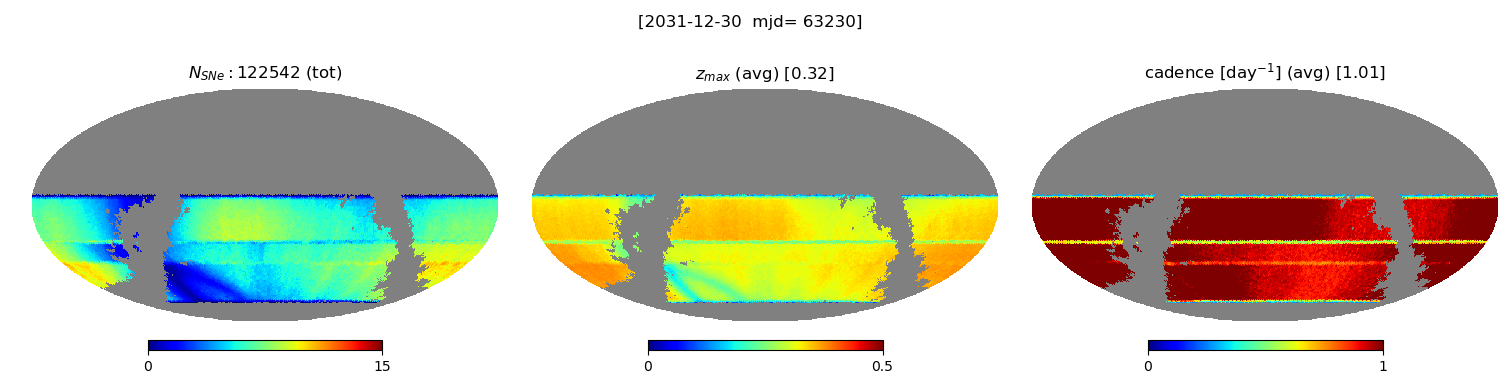
\includegraphics[width=\linewidth]{wfd_maps/altsched_rolling_good_weather_64_maps.png}
    \caption{{\bf AltSched rolling} cadence: {\em Left:} total number
      of well sampled SNe~Ia per healpixel {\em center:} average
      maximum redshift at which the normal SN is no longer well
      sampled {\em right:} average cadence delivered by the survey.}
    \label{fig:altsched_rolling_good_weather}
  \end{center}
\end{figure}


\begin{figure}[h!]
  \begin{center}
    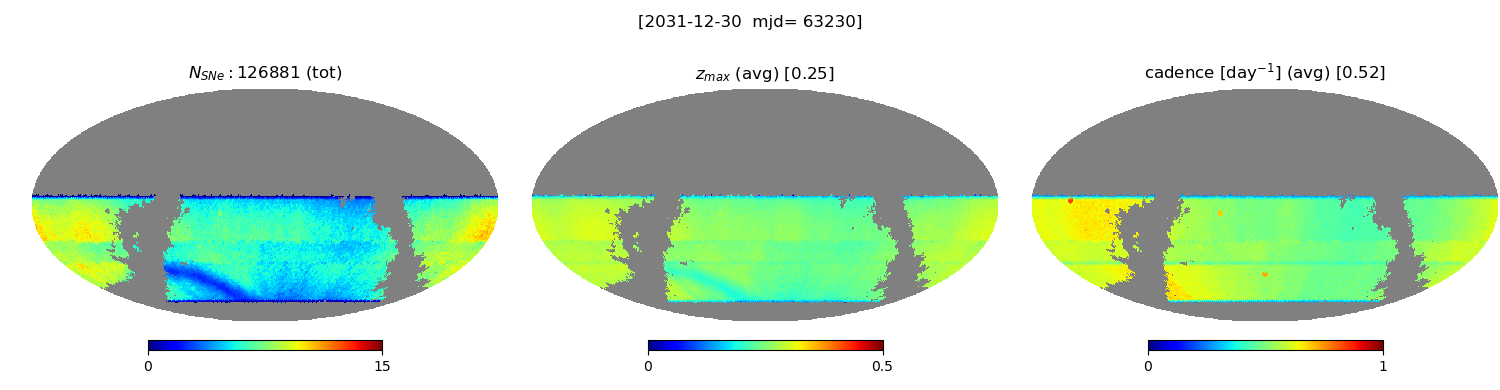
\includegraphics[width=\linewidth]{wfd_maps/altsched_good_weather_64_maps.png}
    \caption{{\bf AltSched} cadence: {\em Left:} total number of well
      sampled SNe~Ia per healpixel {\em center:} average maximum
      redshift at which the normal SN is no longer well sampled {\em
        right:} average cadence delivered by the survey.}
    \label{fig:altsched_good_weather}
  \end{center}
\end{figure}

\begin{figure}[h!]
  \begin{center}
    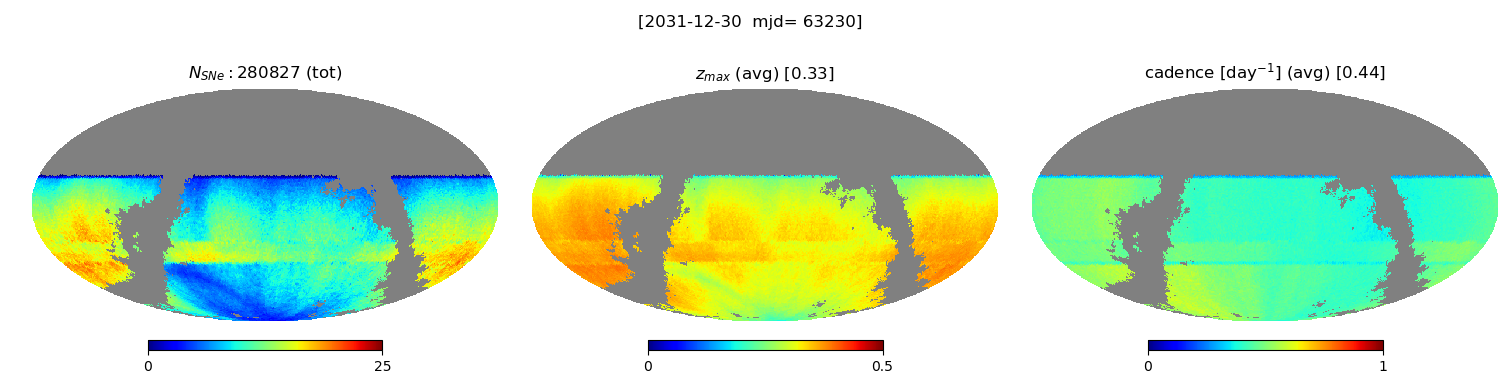
\includegraphics[width=\linewidth]{wfd_maps/altsched_18__90_40_64_maps.png}
    \caption{{\bf AltSched Wide} cadence: {\em Left:} total number of well
      sampled SNe~Ia per healpixel {\em center:} average maximum
      redshift at which the normal SN is no longer well sampled {\em
        right:} average cadence delivered by the survey.}
  \end{center}
  \label{fig:altsched_wide}
\end{figure}

\begin{figure}[h!]
  \begin{center}
    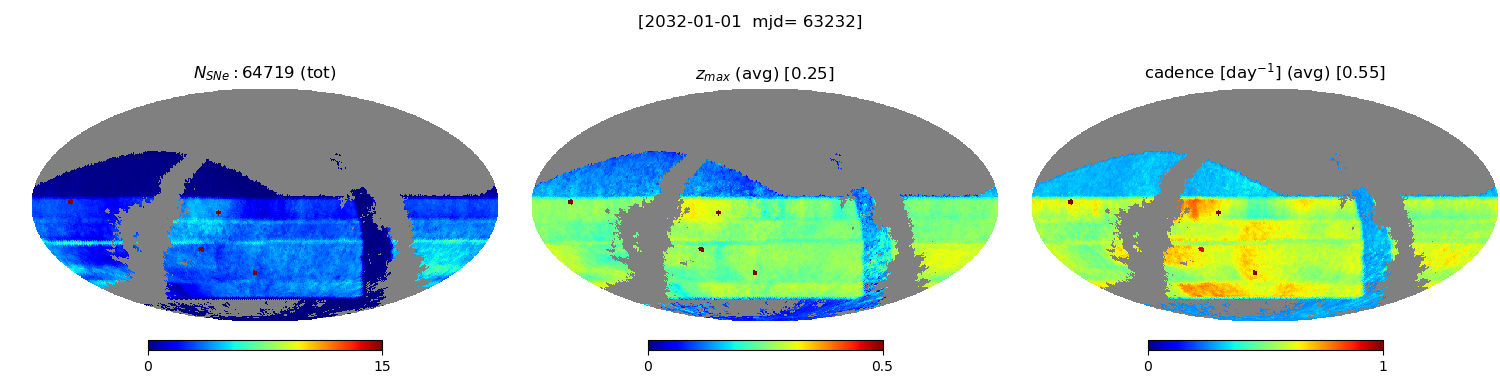
\includegraphics[width=\linewidth]{wfd_maps/tms_roll_10yrs_64_maps.png}
    \caption{{\bf SLAIR tms roll} cadence: {\em Left:} total number of well
      sampled SNe~Ia per healpixel {\em center:} average maximum
      redshift at which the normal SN is no longer well sampled {\em
        right:} average cadence delivered by the survey.}
    \label{fig:tms_roll}
  \end{center}
\end{figure}

\begin{figure}[h!]
  \begin{center}
    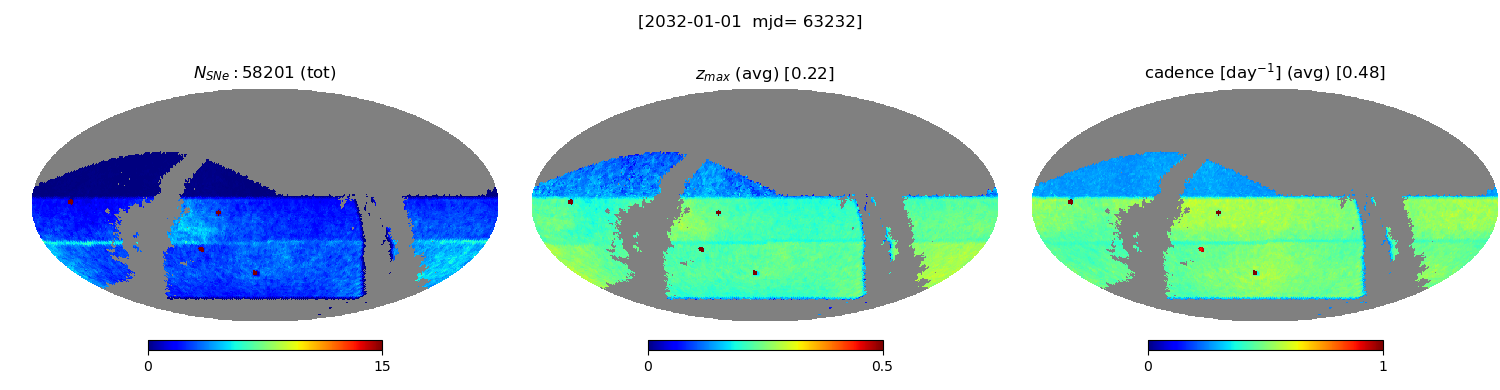
\includegraphics[width=\linewidth]{wfd_maps/rolling_mix_75_10yrs_64_maps.png}
    \caption{{\bf SLAIR: rolling mix 75} cadence: {\em Left:} total number of well
      sampled SNe~Ia per healpixel {\em center:} average maximum
      redshift at which the normal SN is no longer well sampled {\em
        right:} average cadence delivered by the survey.}
    \label{fig:rolling_mix_75}
  \end{center}
\end{figure}


\begin{figure}[h!]
  \begin{center}
    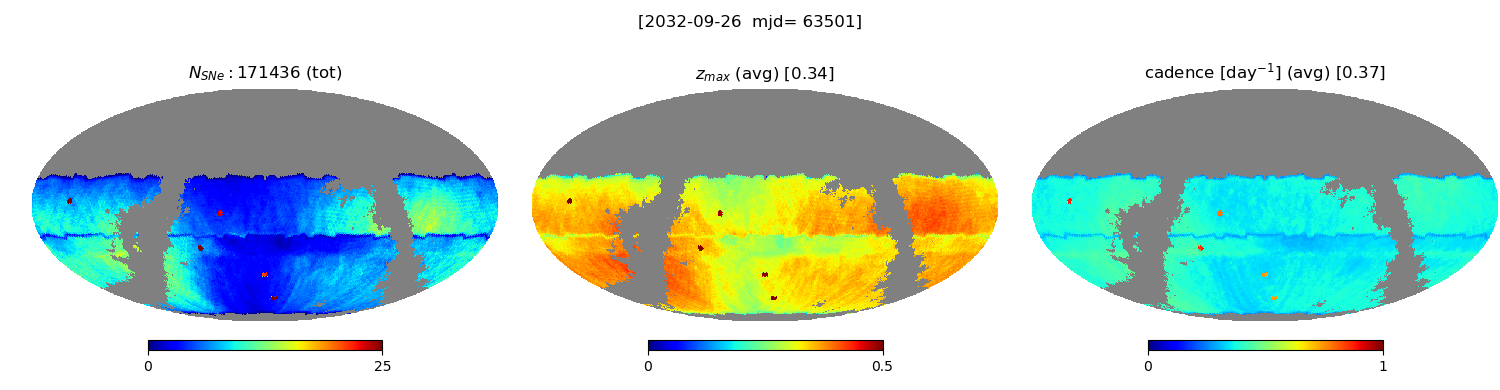
\includegraphics[width=\linewidth]{wfd_maps/mothra_2049_64_maps.png}
    \caption{{\bf Mothra 2049} cadence: {\em Left:} total number of well
      sampled SNe~Ia per healpixel {\em center:} average maximum
      redshift at which the normal SN is no longer well sampled {\em
        right:} average cadence delivered by the survey.}
    \label{fig:mothra_2049}
  \end{center}
\end{figure}

\begin{figure}[h!]
  \begin{center}
    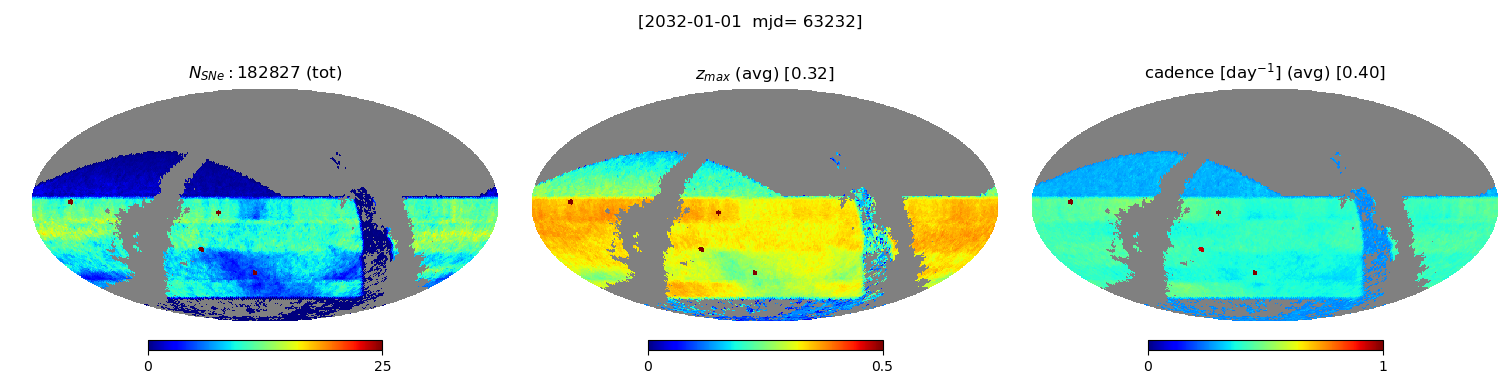
\includegraphics[width=\linewidth]{wfd_maps/tms_drive_10yrs_64_maps.png}
    \caption{{\bf SLAIR tms drive} cadence: {\em Left:} total number of well
      sampled SNe~Ia per healpixel {\em center:} average maximum
      redshift at which the normal SN is no longer well sampled {\em
        right:} average cadence delivered by the survey.}
    \label{fig:tms_drive}
  \end{center}
\end{figure}

\begin{figure}[h!]
  \begin{center}
    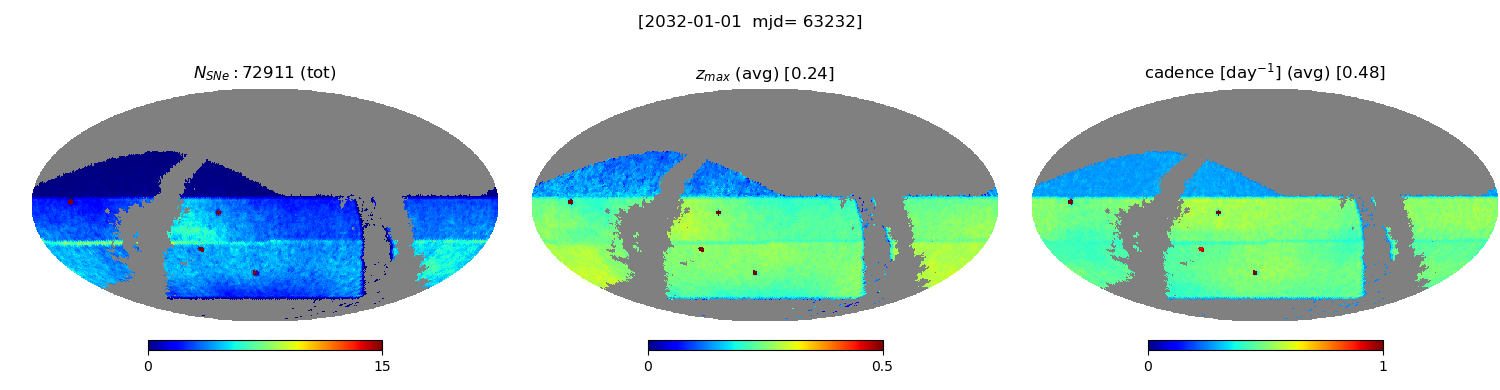
\includegraphics[width=\linewidth]{wfd_maps/rolling_mix_10yrs_64_maps.png}
    \caption{{\bf SLAIR: rolling mix} cadence: {\em Left:} total number of well
      sampled SNe~Ia per healpixel {\em center:} average maximum
      redshift at which the normal SN is no longer well sampled {\em
        right:} average cadence delivered by the survey.}
    \label{fig:rolling_mix}
  \end{center}
\end{figure}

\begin{figure}[h!]
  \begin{center}
    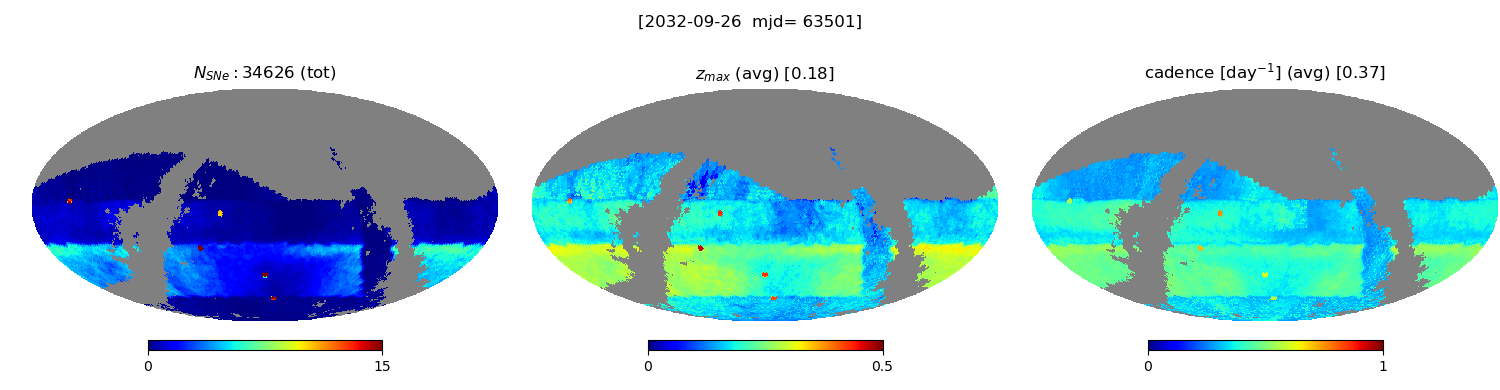
\includegraphics[width=\linewidth]{wfd_maps/mothra_2045_64_maps.png}
    \caption{{\bf Mothra 2045} cadence: {\em Left:} total number of well
      sampled SNe~Ia per healpixel {\em center:} average maximum
      redshift at which the normal SN is no longer well sampled {\em
        right:} average cadence delivered by the survey.}
    \label{fig:mothra_2045}
  \end{center}
\end{figure}

\begin{figure}[h!]
  \begin{center}
    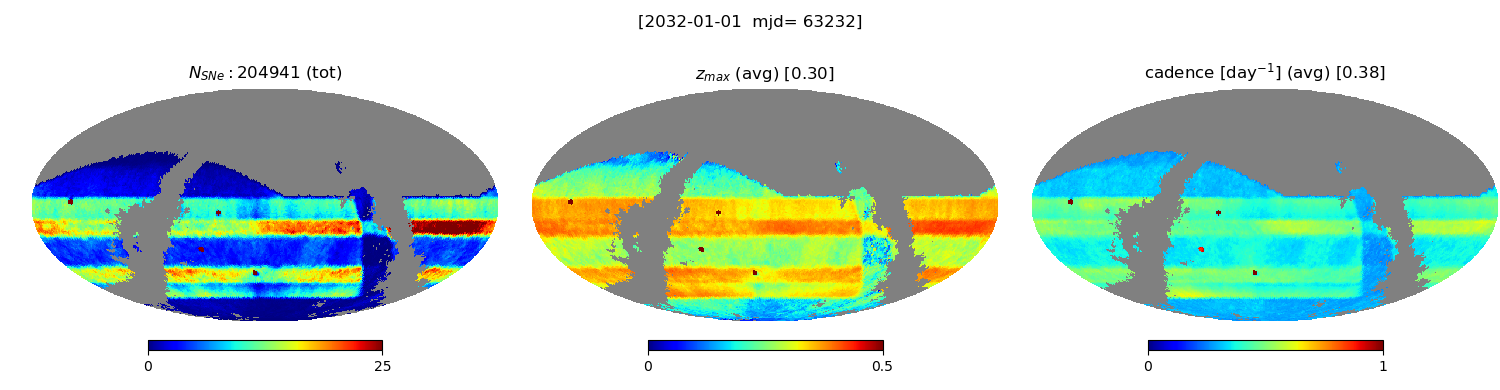
\includegraphics[width=\linewidth]{wfd_maps/tight_mask_10yrs_64_maps.png}
    \caption{{\bf SLAIR tight mask} cadence: {\em Left:} total number of well
      sampled SNe~Ia per healpixel {\em center:} average maximum
      redshift at which the normal SN is no longer well sampled {\em
        right:} average cadence delivered by the survey.}
    \label{fig:tight_mask}
  \end{center}
\end{figure}

\begin{figure}[h!]
  \begin{center}
    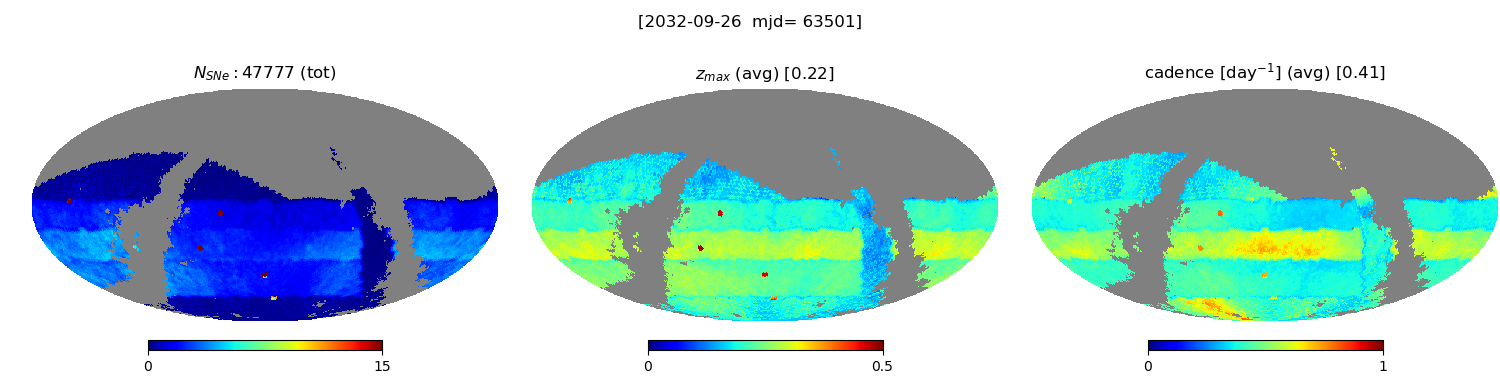
\includegraphics[width=\linewidth]{wfd_maps/kraken_2036_64_maps.png}
    \caption{{\bf Kraken 2036} cadence: {\em Left:} total number of well
      sampled SNe~Ia per healpixel {\em center:} average maximum
      redshift at which the normal SN is no longer well sampled {\em
        right:} average cadence delivered by the survey.}
    \label{fig:kraken_2036}
  \end{center}
\end{figure}

\begin{figure}[h!]
  \begin{center}
    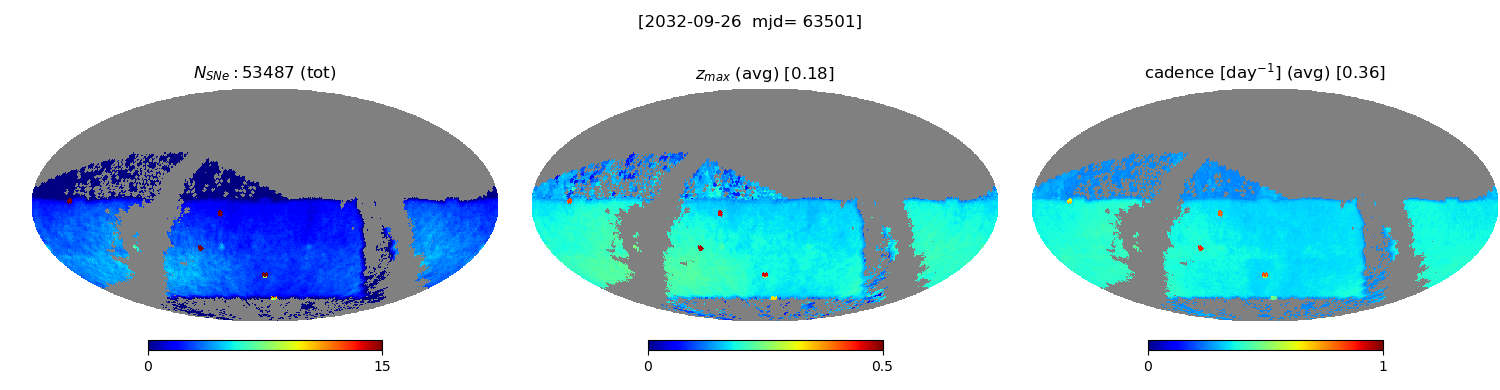
\includegraphics[width=\linewidth]{wfd_maps/pontus_2489_64_maps.png}
    \caption{{\bf Pontus 2489} cadence: {\em Left:} total number of well
      sampled SNe~Ia per healpixel {\em center:} average maximum
      redshift at which the normal SN is no longer well sampled {\em
        right:} average cadence delivered by the survey.}
    \label{fig:pontus_2489}
  \end{center}
\end{figure}

\begin{figure}[h!]
  \begin{center}
    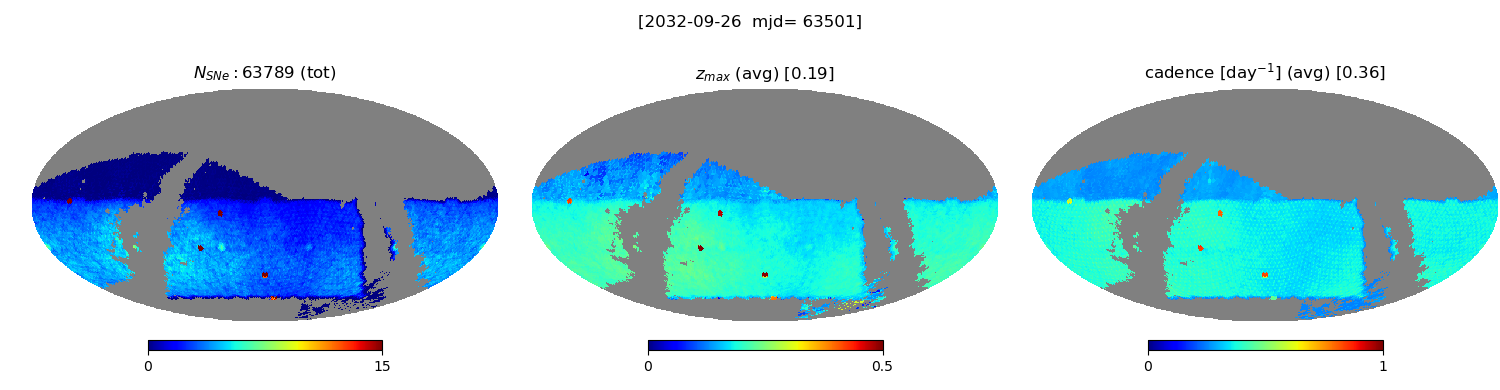
\includegraphics[width=\linewidth]{wfd_maps/colossus_2667_64_maps.png}
    \caption{{\bf Colossus 2667} cadence: {\em Left:} total number of well
      sampled SNe~Ia per healpixel {\em center:} average maximum
      redshift at which the normal SN is no longer well sampled {\em
        right:} average cadence delivered by the survey.}
  \end{center}
  \label{fig:colossus_2667}
\end{figure}

\begin{figure}[h!]
  \begin{center}
    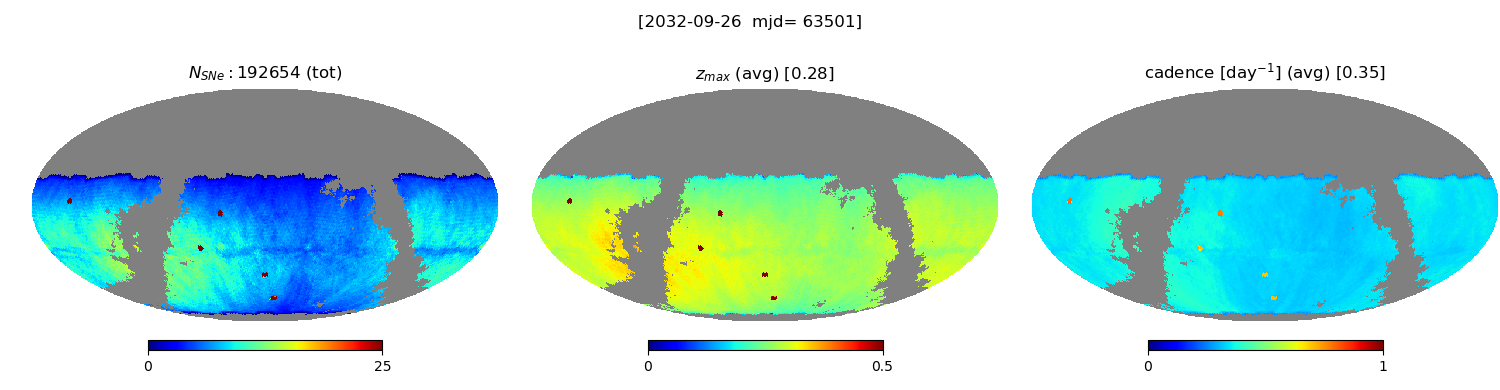
\includegraphics[width=\linewidth]{wfd_maps/kraken_2044_64_maps.png}
    \caption{{\bf Kraken 2044} cadence: {\em Left:} total number of well
      sampled SNe~Ia per healpixel {\em center:} average maximum
      redshift at which the normal SN is no longer well sampled {\em
        right:} average cadence delivered by the survey.}
    \label{fig:kraken_2044}
  \end{center}
\end{figure}

\begin{figure}[h!]
  \begin{center}
    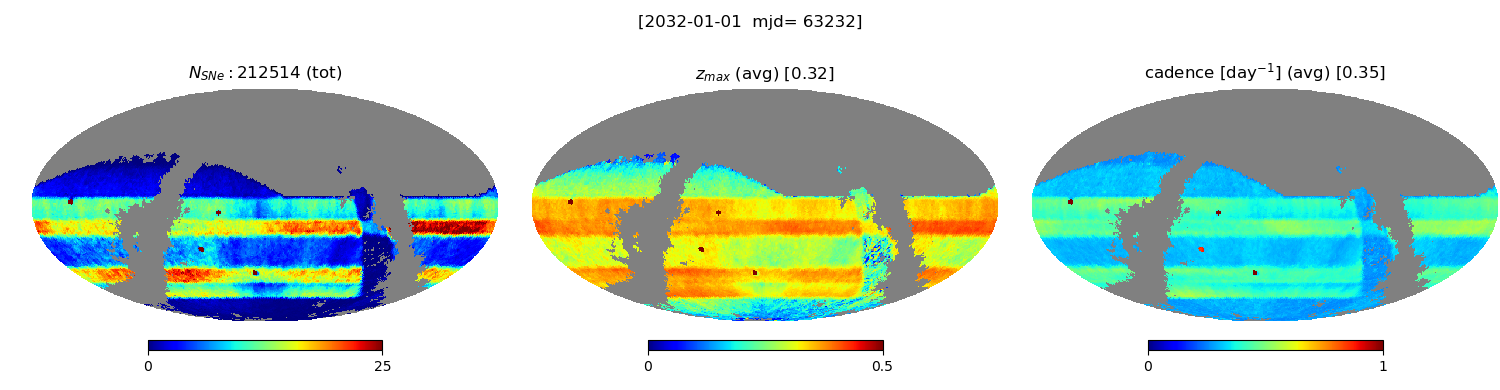
\includegraphics[width=\linewidth]{wfd_maps/tight_mask_simple_10yrs_64_maps.png}
    \caption{{\bf SLAIR tight mask simple} cadence: {\em Left:} total number of well
      sampled SNe~Ia per healpixel {\em center:} average maximum
      redshift at which the normal SN is no longer well sampled {\em
        right:} average cadence delivered by the survey.}
    \label{fig:tight_mask_simple}
  \end{center}
\end{figure}

\begin{figure}[h!]
  \begin{center}
    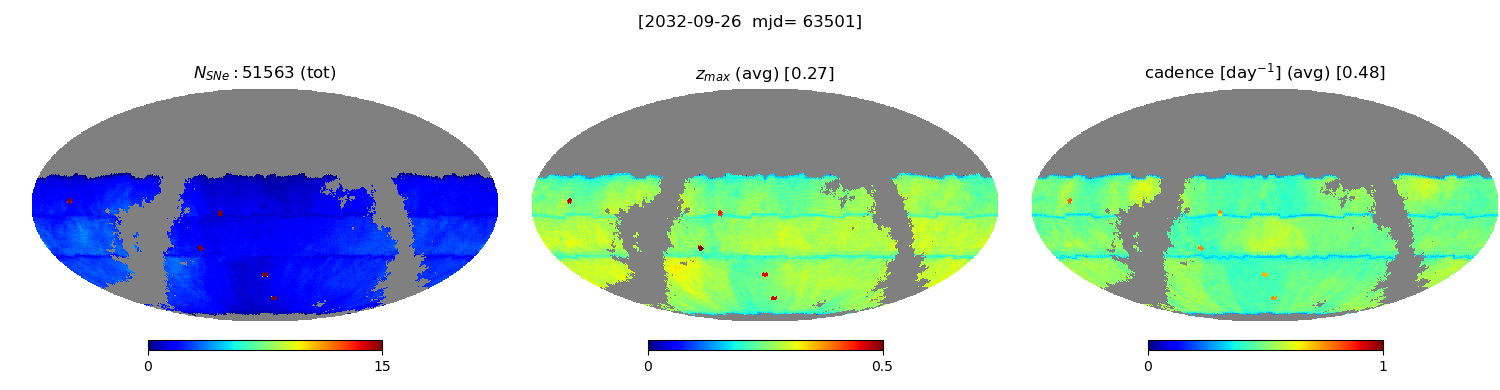
\includegraphics[width=\linewidth]{wfd_maps/nexus_2097_64_maps.png}
    \caption{{\bf Nexus 2097} cadence: {\em Left:} total number of well
      sampled SNe~Ia per healpixel {\em center:} average maximum
      redshift at which the normal SN is no longer well sampled {\em
        right:} average cadence delivered by the survey.}
    \label{fig:nexus_2097}
  \end{center}
\end{figure}

\begin{figure}[h!]
  \begin{center}
    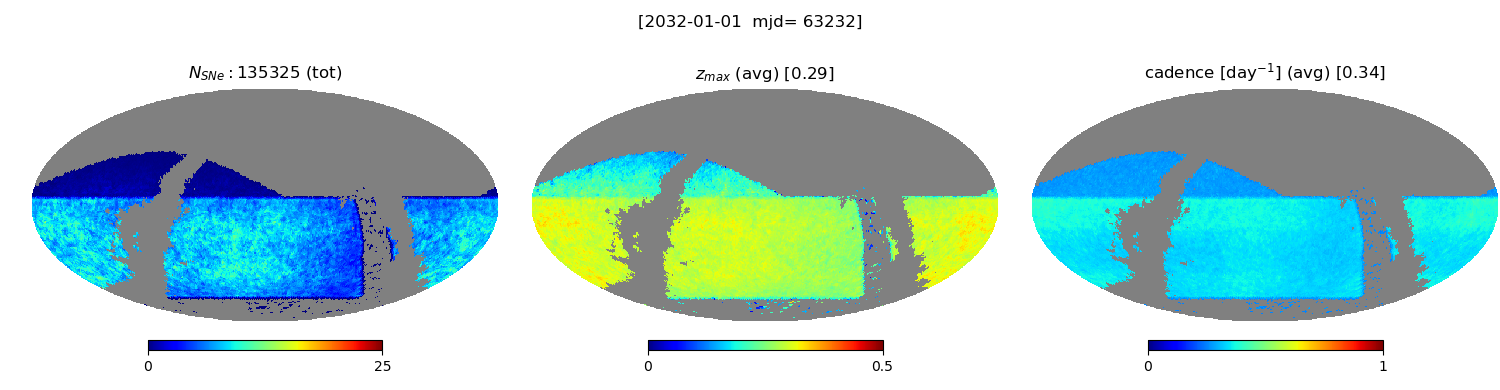
\includegraphics[width=\linewidth]{wfd_maps/cadence_mix_10yrs_64_maps.png}
    \caption{{\bf SLAIR: mix} cadence: {\em Left:} total number of well
      sampled SNe~Ia per healpixel {\em center:} average maximum
      redshift at which the normal SN is no longer well sampled {\em
        right:} average cadence delivered by the survey.}
    \label{fig:cadence_mix}
  \end{center}
\end{figure}

\begin{figure}[h!]
  \begin{center}
    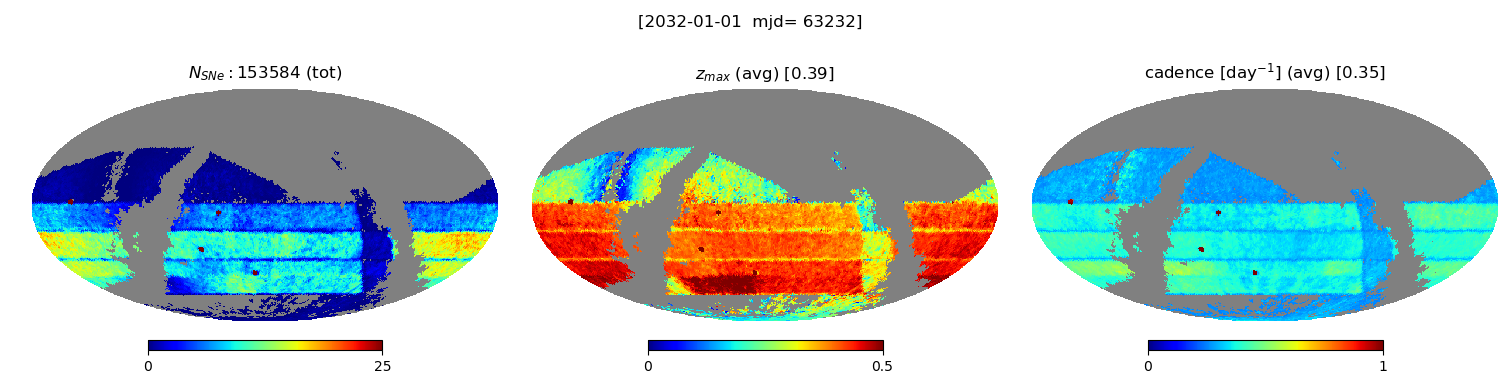
\includegraphics[width=\linewidth]{wfd_maps/feature_rolling_twoThird_10yrs_64_maps.png}
    \caption{{\bf Feature rolling 2/3} cadence: {\em Left:} total number of well
      sampled SNe~Ia per healpixel {\em center:} average maximum
      redshift at which the normal SN is no longer well sampled {\em
        right:} average cadence delivered by the survey.}
    \label{fig:feature_rolling_two_third}
  \end{center}
\end{figure}

\begin{figure}[h!]
  \begin{center}
    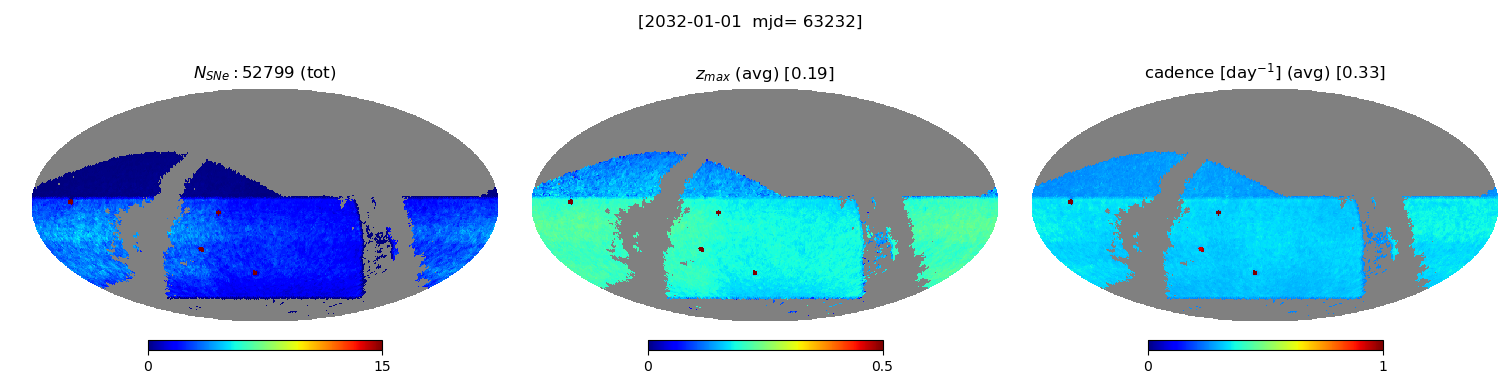
\includegraphics[width=\linewidth]{wfd_maps/blobs_mix_zmask10yrs_64_maps.png}
    \caption{{\bf SLAIR: blobs mix zmask} cadence: {\em Left:} total number of well
      sampled SNe~Ia per healpixel {\em center:} average maximum
      redshift at which the normal SN is no longer well sampled {\em
        right:} average cadence delivered by the survey.}
    \label{fig:blobs_mix_zmask}
  \end{center}
\end{figure}

\begin{figure}[h!]
  \begin{center}
    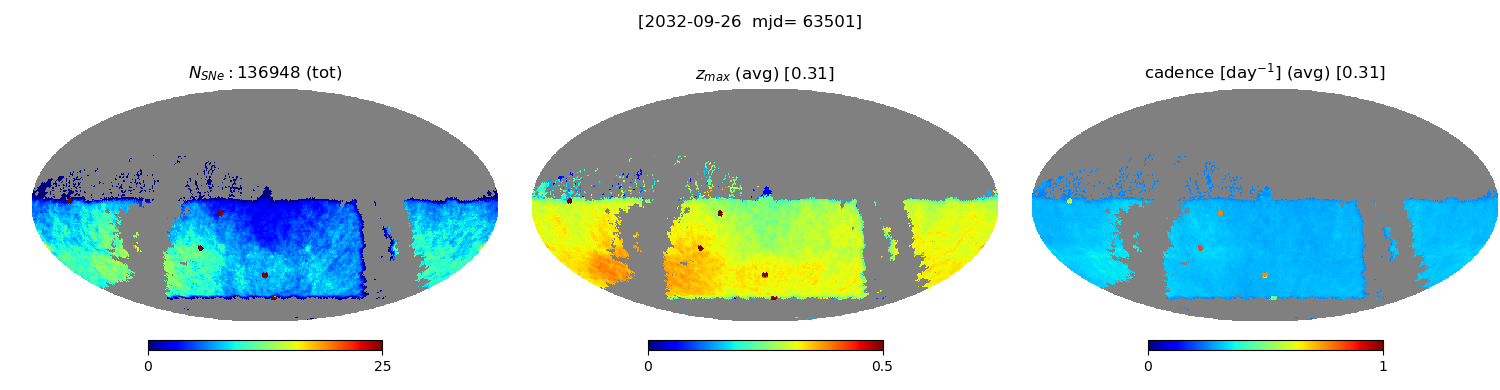
\includegraphics[width=\linewidth]{wfd_maps/kraken_2026_64_maps.png}
    \caption{{\bf Kraken 2026} cadence: {\em Left:} total number of well
      sampled SNe~Ia per healpixel {\em center:} average maximum
      redshift at which the normal SN is no longer well sampled {\em
        right:} average cadence delivered by the survey.}
  \end{center}
  \label{fig:kraken_2026}
\end{figure}

\begin{figure}[h!]
  \begin{center}
    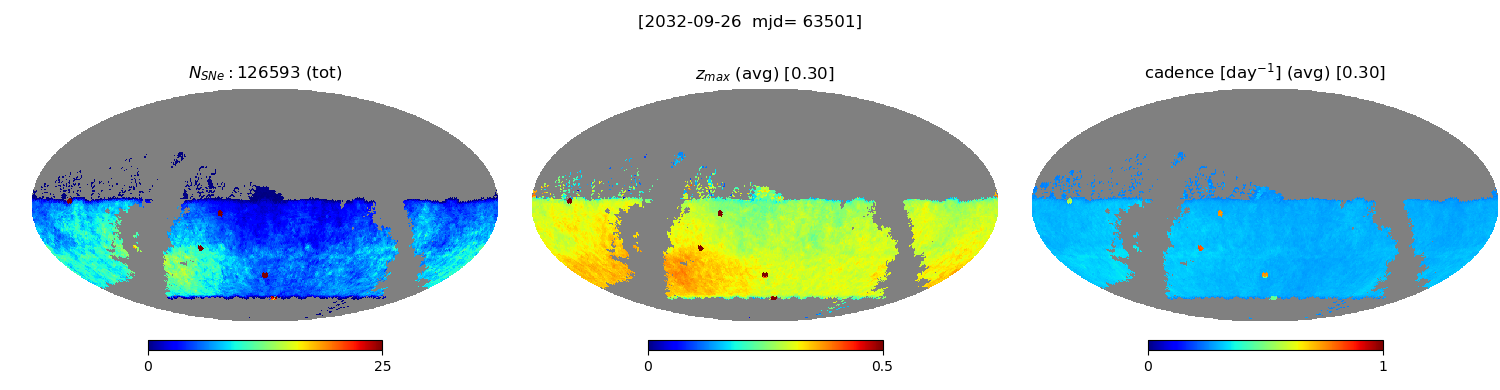
\includegraphics[width=\linewidth]{wfd_maps/colossus_2664_64_maps.png}
    \caption{{\bf Colossus 2664} cadence: {\em Left:} total number of well
      sampled SNe~Ia per healpixel {\em center:} average maximum
      redshift at which the normal SN is no longer well sampled {\em
        right:} average cadence delivered by the survey.}
    \label{fig:colossus_2664}
  \end{center}
\end{figure}

\begin{figure}[h!]
  \begin{center}
    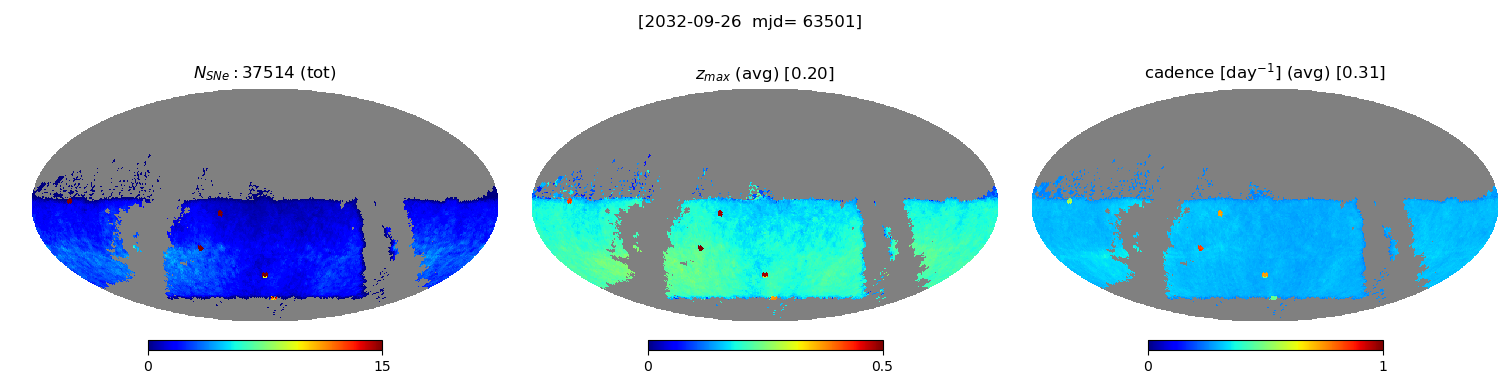
\includegraphics[width=\linewidth]{wfd_maps/baseline2018a_64_maps.png}
    \caption{{\bf Baseline 2018a} cadence: {\em Left:} total number of well
      sampled SNe~Ia per healpixel {\em center:} average maximum
      redshift at which the normal SN is no longer well sampled {\em
        right:} average cadence delivered by the survey.}
  \end{center}
  \label{fig:baseline2018}
\end{figure}

\begin{figure}[h!]
  \begin{center}
    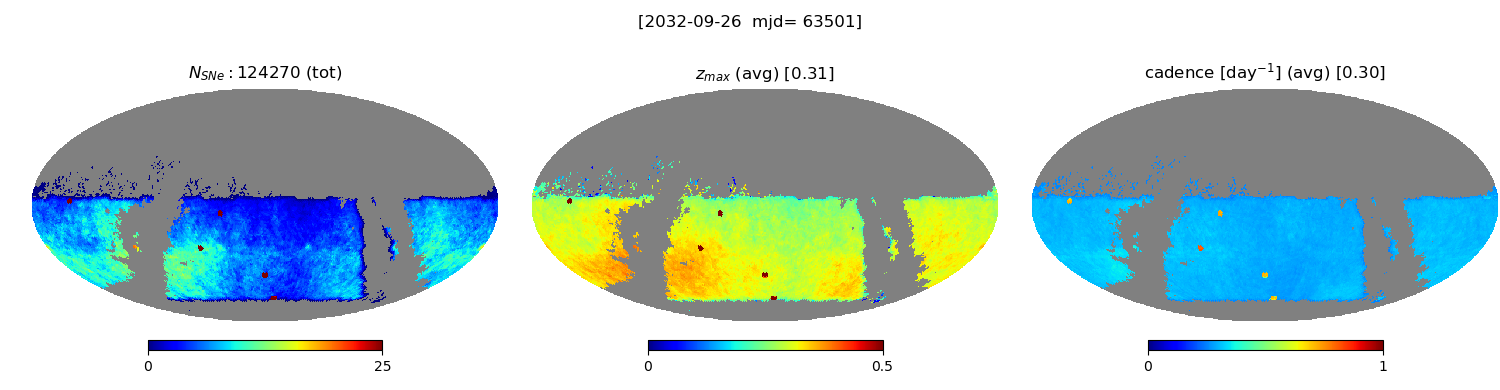
\includegraphics[width=\linewidth]{wfd_maps/colossus_2665_64_maps.png}
    \caption{{\bf Colossus 2665} cadence: {\em Left:} total number of well
      sampled SNe~Ia per healpixel {\em center:} average maximum
      redshift at which the normal SN is no longer well sampled {\em
        right:} average cadence delivered by the survey.}
  \end{center}
  \label{fig:colossus_2665}
\end{figure}

\begin{figure}[h!]
  \begin{center}
    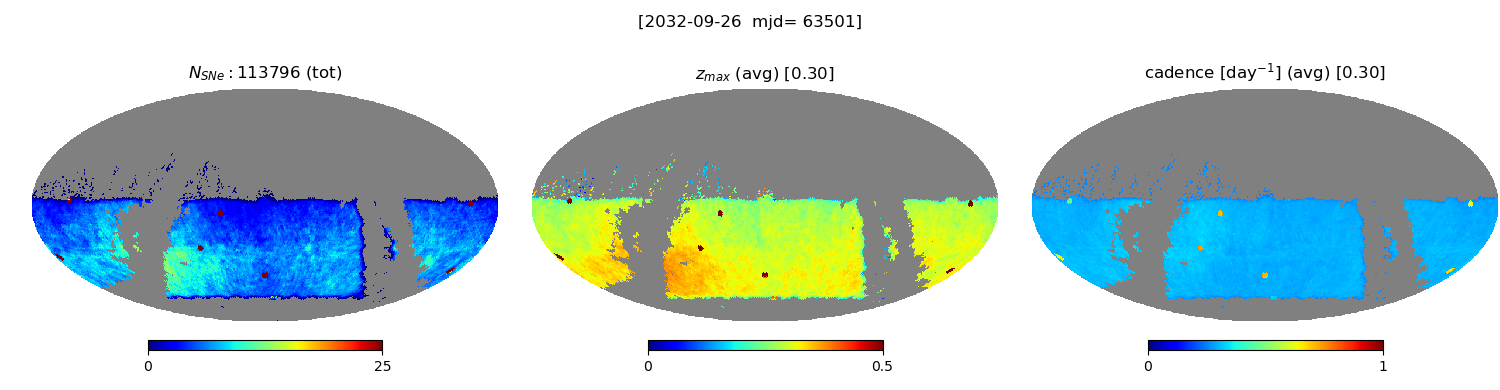
\includegraphics[width=\linewidth]{wfd_maps/kraken_2035_64_maps.png}
    \caption{{\bf Kraken 2035} cadence: {\em Left:} total number of well
      sampled SNe~Ia per healpixel {\em center:} average maximum
      redshift at which the normal SN is no longer well sampled {\em
        right:} average cadence delivered by the survey.}
  \end{center}
  \label{fig:kraken_2035}
\end{figure}

\begin{figure}[h!]
  \begin{center}
    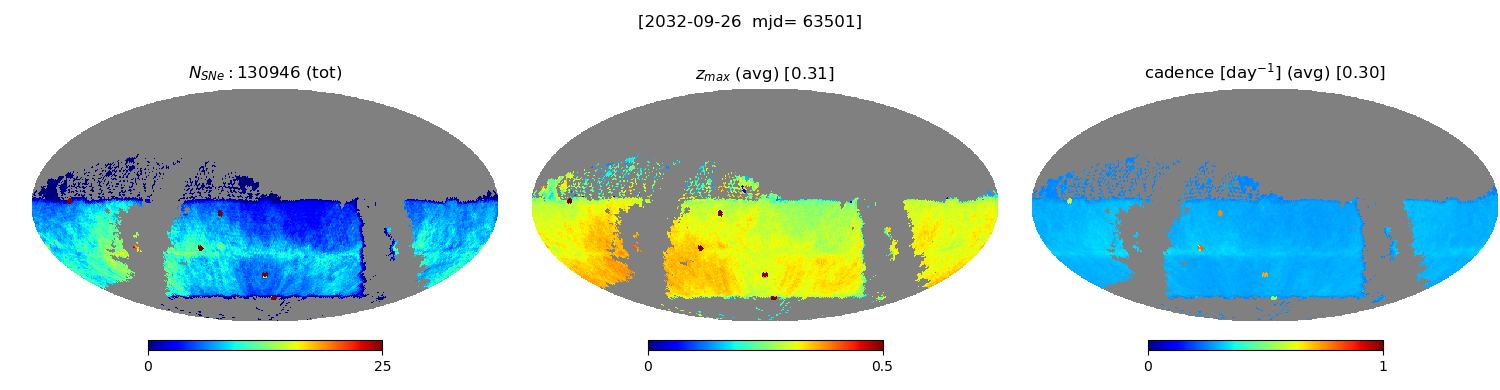
\includegraphics[width=\linewidth]{wfd_maps/kraken_2042_64_maps.png}
    \caption{{\bf Kraken 2042} cadence: {\em Left:} total number of well
      sampled SNe~Ia per healpixel {\em center:} average maximum
      redshift at which the normal SN is no longer well sampled {\em
        right:} average cadence delivered by the survey.}
    \label{fig:kraken_2042}
  \end{center}
\end{figure}

\begin{figure}[h!]
  \begin{center}
    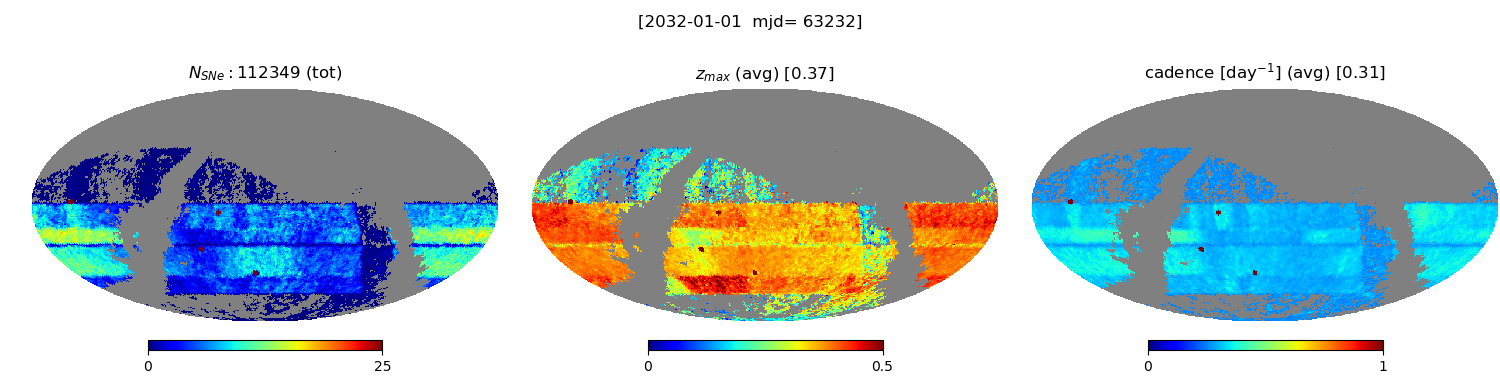
\includegraphics[width=\linewidth]{wfd_maps/feature_rolling_half_mask_10yrs_64_maps.png}
    \caption{{\bf Feature rolling 1/2} cadence: {\em Left:} total number of well
      sampled SNe~Ia per healpixel {\em center:} average maximum
      redshift at which the normal SN is no longer well sampled {\em
        right:} average cadence delivered by the survey.}
    \label{fig:feature_rolling_half_mask}
  \end{center}
\end{figure}


\begin{figure}[h!]
  \begin{center}
    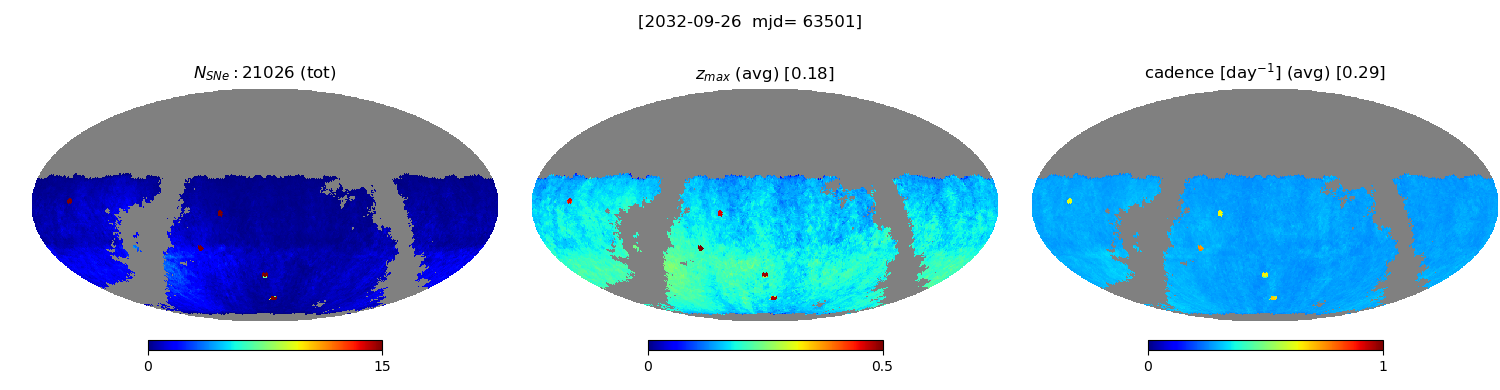
\includegraphics[width=\linewidth]{wfd_maps/pontus_2002_64_maps.png}
    \caption{{\bf Pontus 2002} cadence: {\em Left:} total number of well
      sampled SNe~Ia per healpixel {\em center:} average maximum
      redshift at which the normal SN is no longer well sampled {\em
        right:} average cadence delivered by the survey.}
    \label{fig:pontus_2002}
  \end{center}
\end{figure}

\begin{figure}[h!]
  \begin{center}
    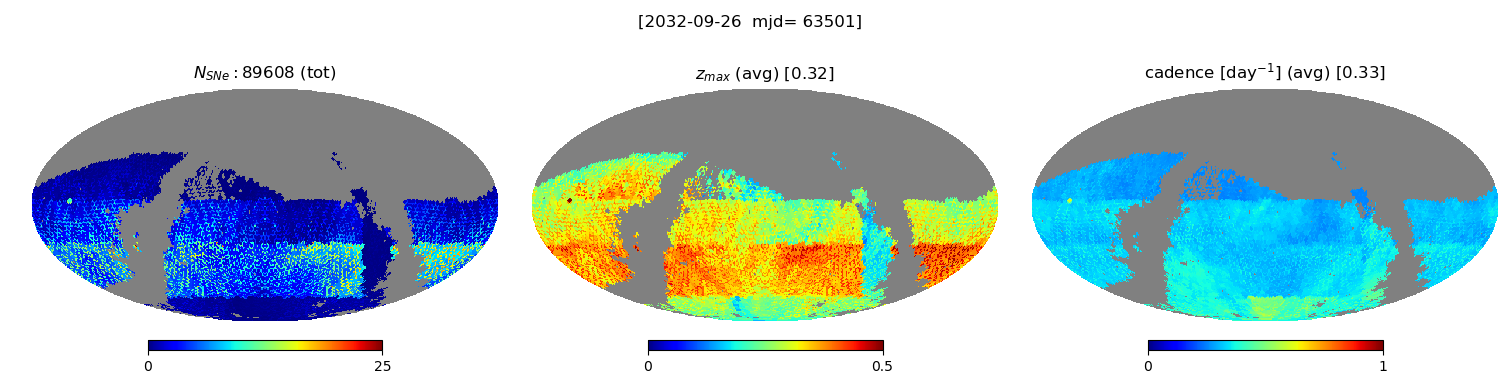
\includegraphics[width=\linewidth]{wfd_maps/pontus_2502_64_maps.png}
    \caption{{\bf Pontus 2502} cadence: {\em Left:} total number of well
      sampled SNe~Ia per healpixel {\em center:} average maximum
      redshift at which the normal SN is no longer well sampled {\em
        right:} average cadence delivered by the survey.}
    \label{fig:pontus_2502}
  \end{center}
\end{figure}

\begin{figure}[h!]
  \begin{center}
    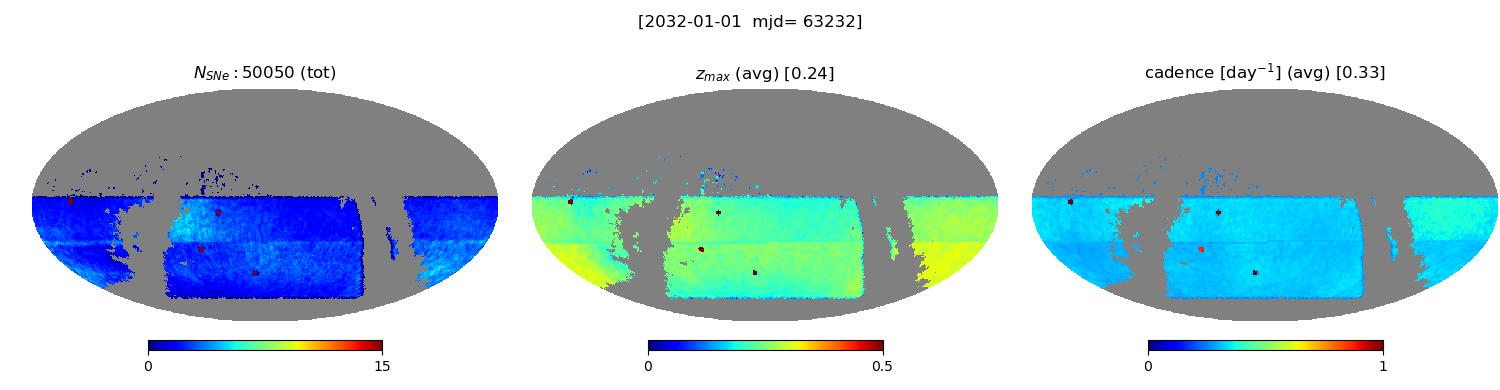
\includegraphics[width=\linewidth]{wfd_maps/rolling_10yrs_64_maps.png}
    \caption{{\bf SLAIR: rolling} cadence: {\em Left:} total number of well
      sampled SNe~Ia per healpixel {\em center:} average maximum
      redshift at which the normal SN is no longer well sampled {\em
        right:} average cadence delivered by the survey.}
    \label{fig:slair_rolling}
  \end{center}
\end{figure}

\begin{figure}[h!]
  \begin{center}
    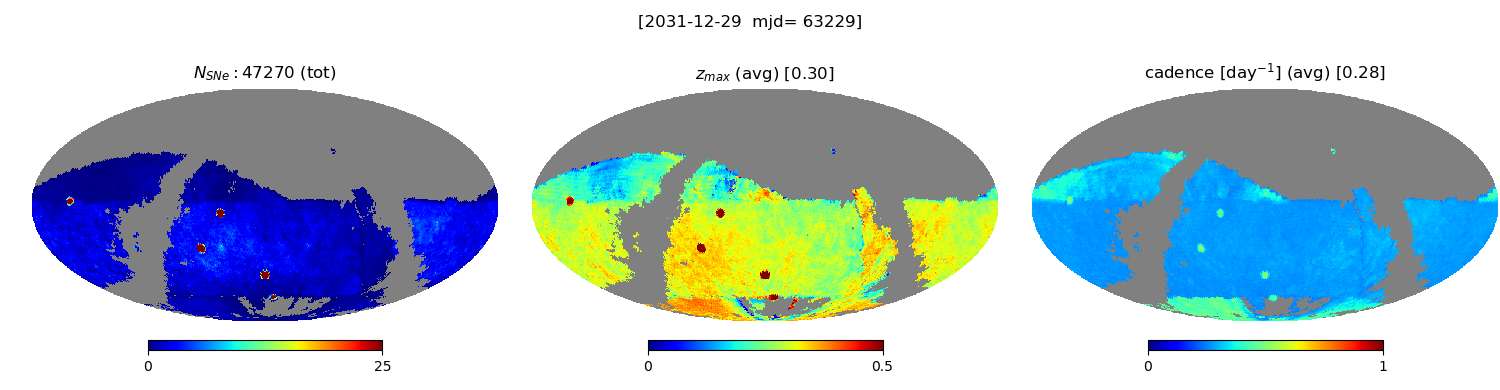
\includegraphics[width=\linewidth]{wfd_maps/minion_1016_64_maps.png}
    \caption{{\bf Minion 1016} cadence: {\em Left:} total number of well
      sampled SNe~Ia per healpixel {\em center:} average maximum
      redshift at which the normal SN is no longer well sampled {\em
        right:} average cadence delivered by the survey.}
    \label{fig:minion_1016}
  \end{center}
\end{figure}

\begin{figure}[h!]
  \begin{center}
    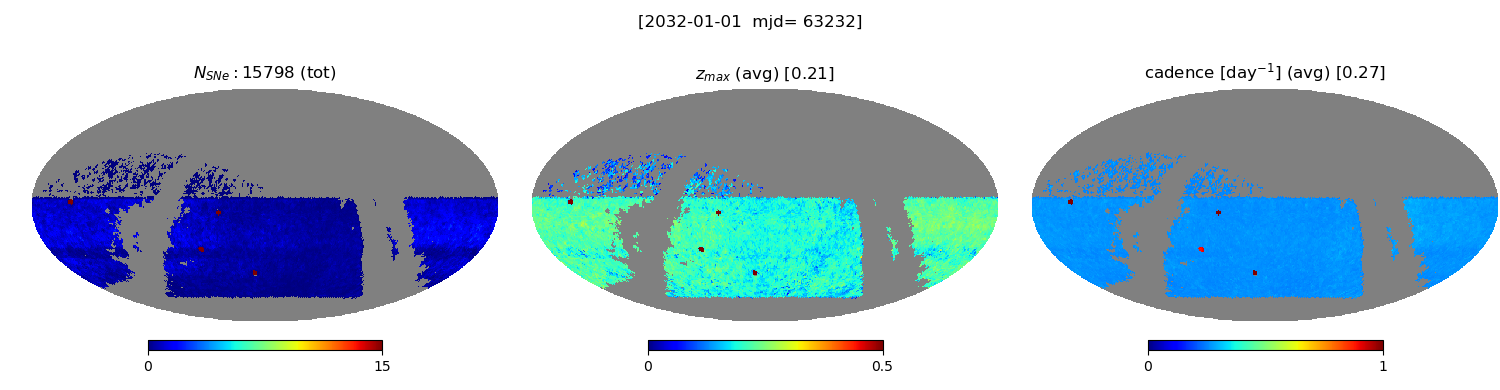
\includegraphics[width=\linewidth]{wfd_maps/blobs_same_10yrs_64_maps.png}
    \caption{{\bf SLAIR: blobs same} cadence: {\em Left:} total number of well
      sampled SNe~Ia per healpixel {\em center:} average maximum
      redshift at which the normal SN is no longer well sampled {\em
        right:} average cadence delivered by the survey.}
    \label{fig:blobs_same}
  \end{center}
\end{figure}

\begin{figure}[h!]
  \begin{center}
    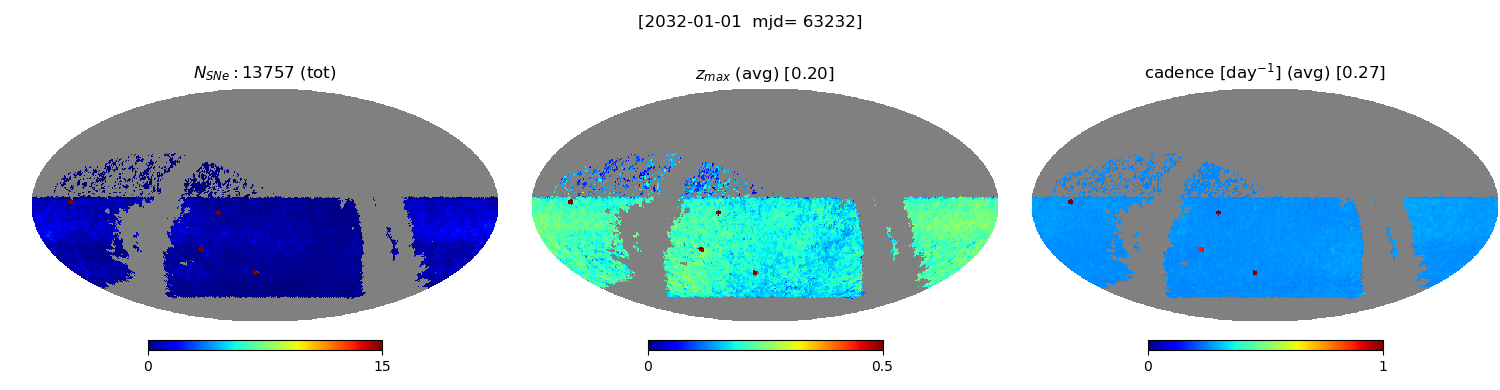
\includegraphics[width=\linewidth]{wfd_maps/blobs_same_zmask10yrs_64_maps.png}
    \caption{{\bf SLAIR: blobs same zmask} cadence: {\em Left:} total number of well
      sampled SNe~Ia per healpixel {\em center:} average maximum
      redshift at which the normal SN is no longer well sampled {\em
        right:} average cadence delivered by the survey.}
    \label{fig:blobs_same_zmask}
  \end{center}
\end{figure}

\begin{figure}[h!]
  \begin{center}
    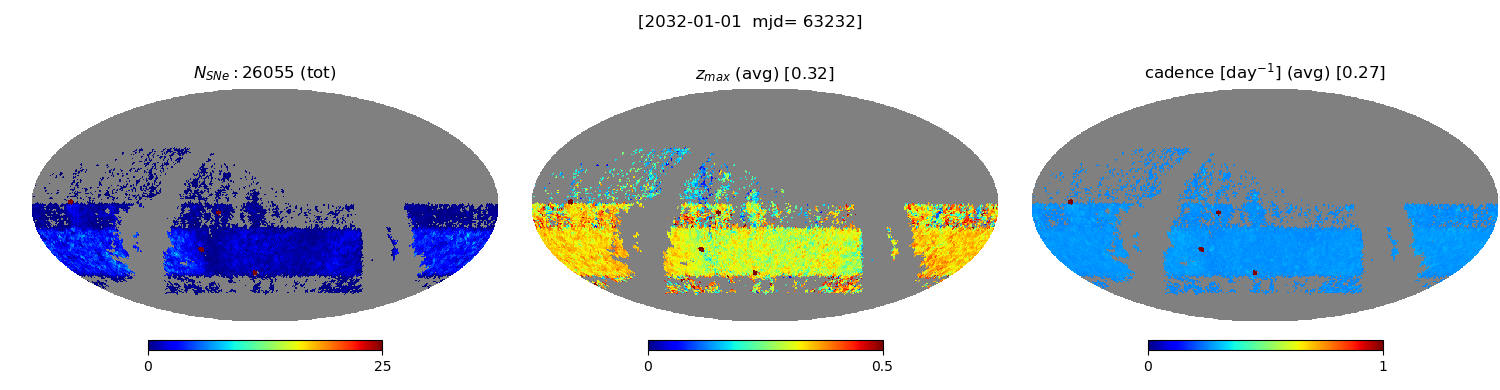
\includegraphics[width=\linewidth]{wfd_maps/feature_baseline_10yrs_64_maps.png}
    \caption{{\bf Feature baseline} cadence: {\em Left:} total number of well
      sampled SNe~Ia per healpixel {\em center:} average maximum
      redshift at which the normal SN is no longer well sampled {\em
        right:} average cadence delivered by the survey.}
    \label{fig:feature_baseline}
  \end{center}
\end{figure}







%\vspace*{20cm}
  
\clearpage

\section{\opsim~and \altsched}
\label{sec:opsim_altsched}

\opsim~and \altsched~schedulers have adopted two different ways of observing the sky. While the former relies on a greedy algorithm to decide which pointing should be performed (optimisation based on slew-time minimisation, optimal observing conditions - in terms of sky brightness and airmass for instance), the latter scans near the meridian dense areas (pre-defined at the begining of the night) of the sky. Fig. \ref{fig:night_comp} illustrate the area observed at the end of a night for both schedulers. One may observe that \altsched~scans dense area of the sky while regions observed by \opsim~are sparsely populated. It may thus be more difficult to ensure a regular cadence with \opsim~method. Both schedulers perform observations near the meridian (Fig. \ref{fig:scan_meridian}).

\begin{figure}[!htbp]
  \centering
  \subfigure[OpSim]{\label{fig:opsim_night}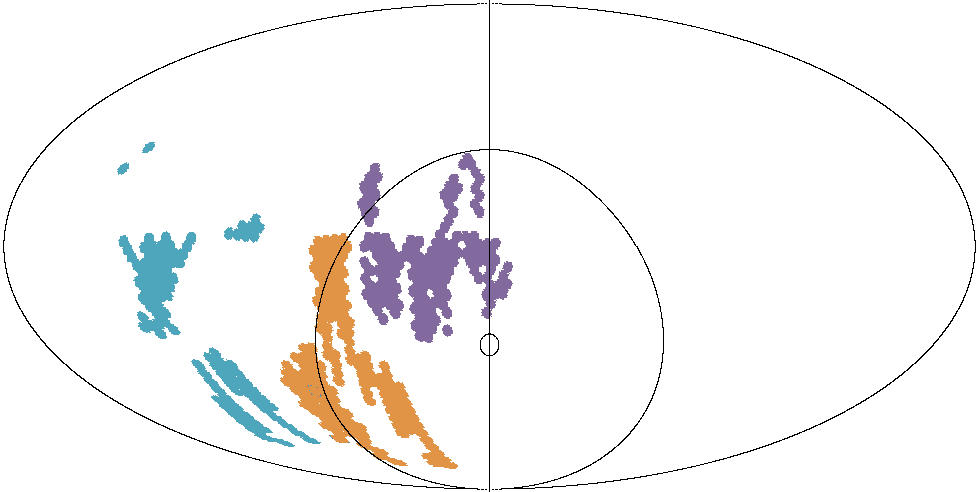
\includegraphics[width=0.8\textwidth]{opsim_vs_altsched/opsim_night.png}}
  \subfigure[altsched]{\label{fig:altsched_night}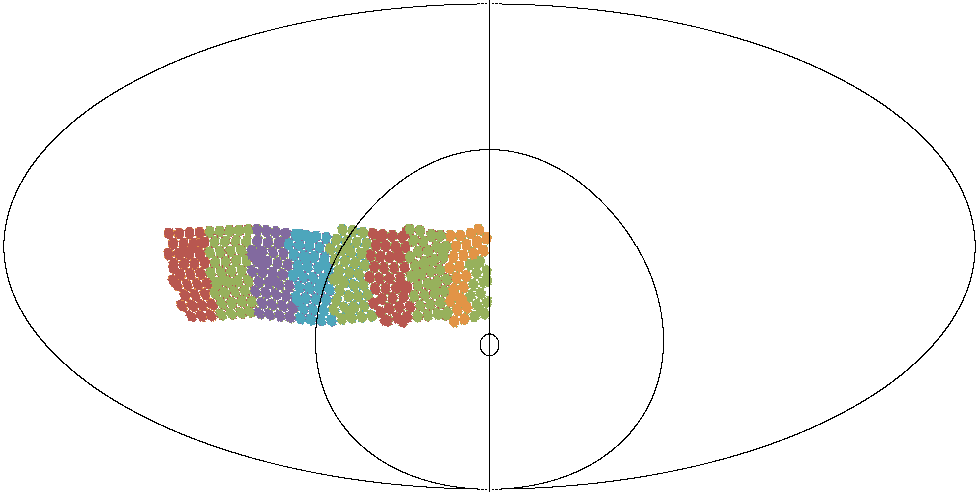
\includegraphics[width=0.8\textwidth]{opsim_vs_altsched/altsched_night.png}}
  \caption{Area coverage at the end of a night for \opsim(top) and \altsched(bottom) schedulers.  Each color point corresponds to a pointing. Colors correspond to the latest filter used.}\label{fig:night_comp}
\end{figure}

\begin{figure}[!htbp]
  \begin{center}
    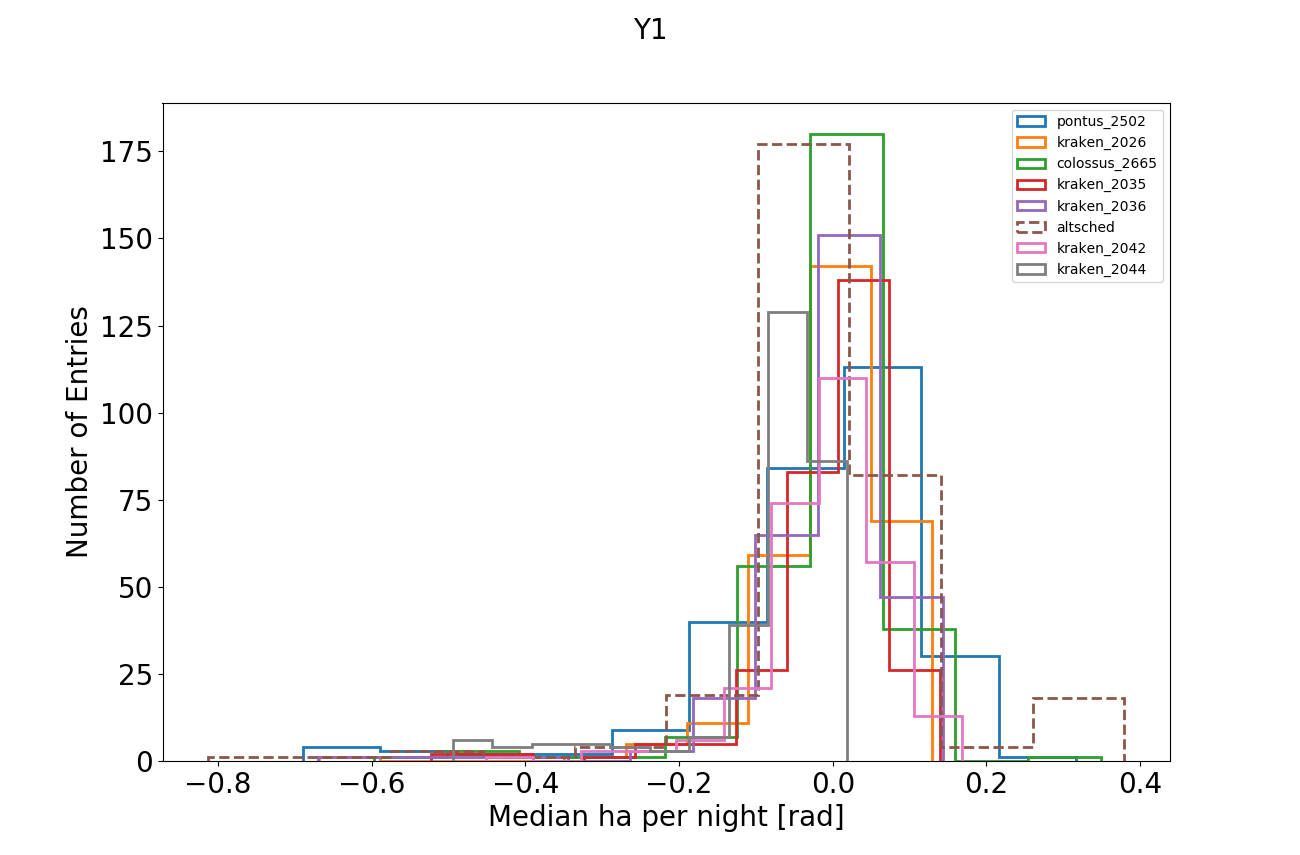
\includegraphics[width=0.7\textwidth]{opsim_vs_altsched/median_ha.png}
    \caption{Median hour angle (first year of the survey) for some of the observing strategies considered in this work.}\label{fig:scan_meridian}
    \end{center}
\end{figure}

One may also observe on Fig. \ref{fig:night_comp} that the filter allocation is quite different between the two schedulers during a night. The number of filter changes per night is indeed higher for \altsched(median value: 12) compared to \opsim(median value: 2) as it can be seen on Fig. \ref{fig:filter_changes}. The global filter allocation (ie the fraction of visits per band after ten years) with \altsched~is not the same in \opsim (see Appendix \ref{sec:globalstat}): in comparison to \opsim~, \altsched~tends to allocate a larger (lower)  number of visits in [u,g,r,z] ([i,y]) bands. This has an impact on \sne~observations in the WFD survey since [g,r,i] are the bands of interest for the redshift range ($z \lesssim 0.4$) accessible.

\begin{figure}[!htbp]
  \begin{center}
    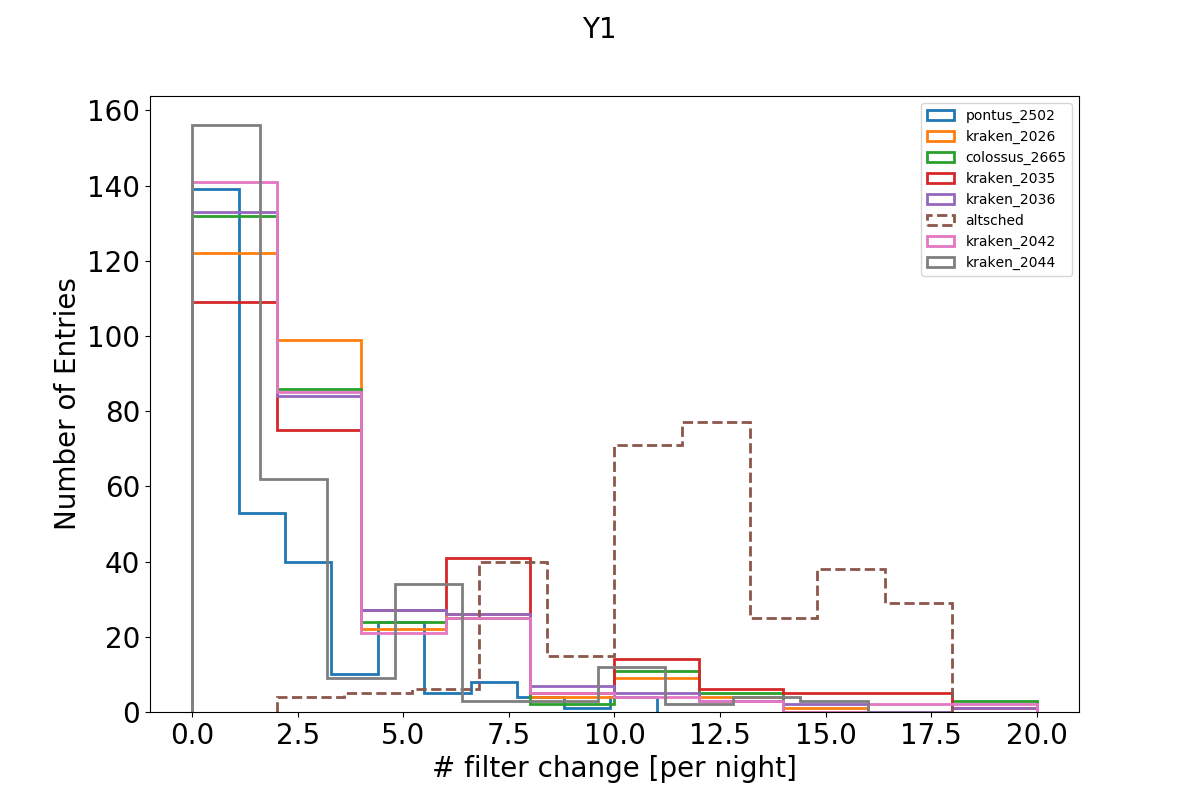
\includegraphics[width=0.7\textwidth]{opsim_vs_altsched/filter_changes.png}
    \caption{Number of filter changes per night (first year of the survey) for some of the observing strategies considered in this work.}\label{fig:filter_changes}
    \end{center}
\end{figure}

A common criticism on \altsched~is that this scheduler allows observations (except in the u-band) when the distance to the Moon is low. While this is true (Fig. \ref{fig:moondist}) one may consider that this correspond to up to ten percent of the total number of visits and that the Moon distance constraint (cut at 30 degrees in \opsim~) may be included in a quite easy way in the code. It would be interesting to run \altsched~simulations including the Moon distance constraint so as to evaluate potential impacts on cadence and filter allocation.

\begin{figure}[!htbp]
  \begin{center}
    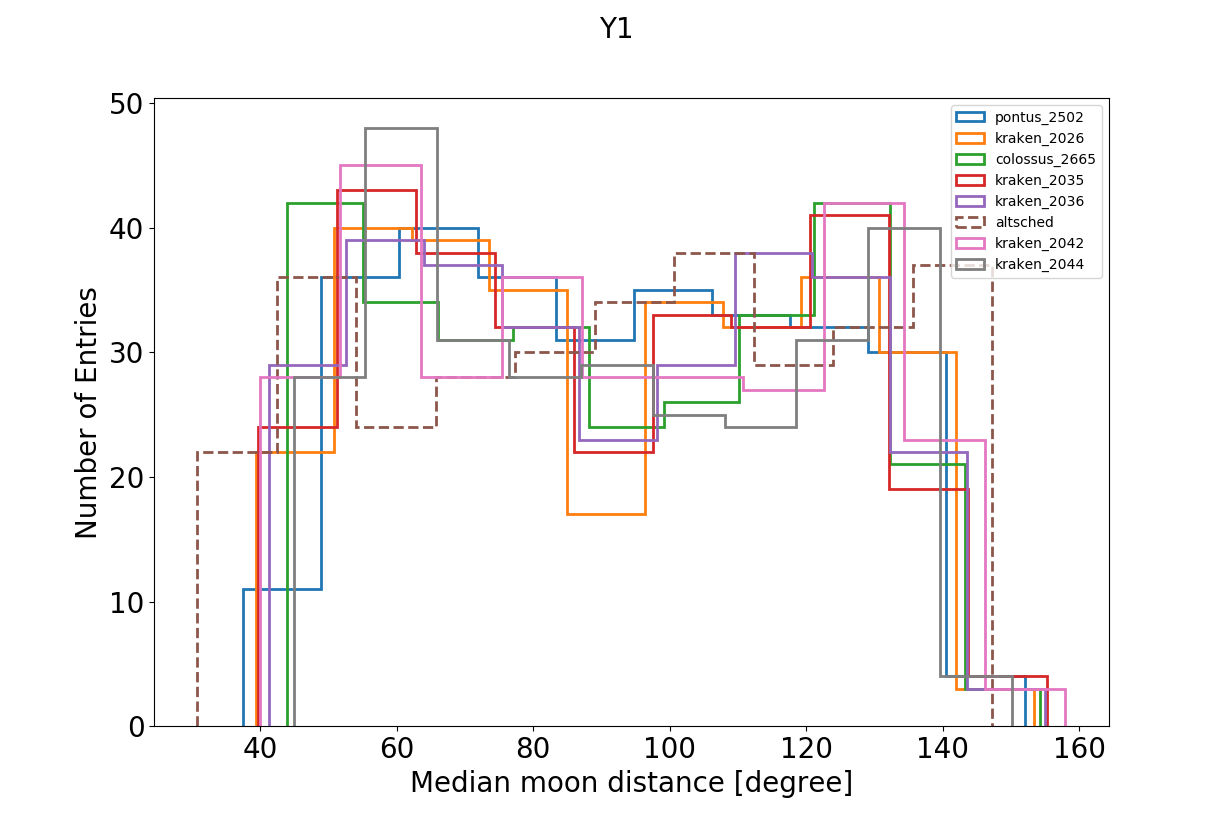
\includegraphics[width=0.7\textwidth]{opsim_vs_altsched/moon_distance.png}
    \caption{Median Moon distance (first year of the survey) for some of the observing strategies considered in this work.}\label{fig:moondist}
    \end{center}
\end{figure}


Finally other differences between the two schedulers include:
\begin{itemize}
\item{DDF} : DDF mini-surveys are not implemented in a coherent way in \altsched. A one hour slot per observing night is allocated to DDF observations but no filter sequence/observations performed during that time.\footnote{This corresponds to versions of the code used to perform the simulations considered in this note. An ongoing work initiated during the LSST Cadence Hackathon (17-19 September 2018; Flatiron Institute, New York, NY) by Daniel Rothchild and Philippe Gris aims at including DDF mini-surveys in a coherent way in \altsched.}
\item{Uncovered area}:  the North Ecliptic Spur, the North Galactic Pole and the South Celestial Pole are not observed by \altsched~.
\item{Galactic Plane}: the Galactic plane is observed by \altsched~in the same way as the WFD survey.

\end{itemize}

A way to quantify the impact of these differences on the main survey (in terms of cadence, filter allocation, ...) would be to ''fake'' these observations (ie allocate time for it with no realistic visit sequence).

One last difference between \opsim~and \altsched concerns the time needed to simulate ten years of survey: it is of about two days for the former and about one to two hours for the latter. There are ongoing efforts in the \opsim team (Peter Yoachim) to minimise this processing time. It is all the more important as a lot of configurations may have to be tested so as to optimize the survey.  


\clearpage

\section{DDF cadence plots}

\begin{figure}[htbp]
\begin{center}
  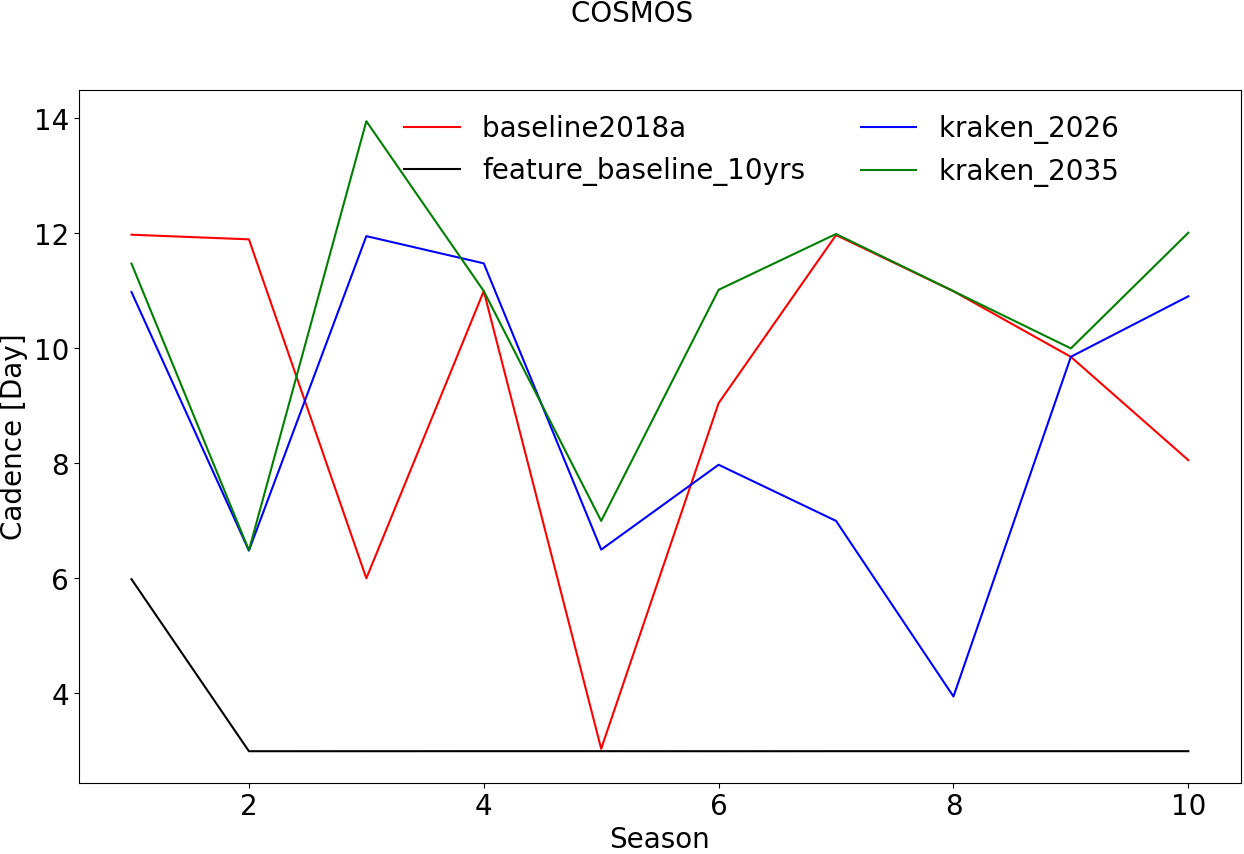
\includegraphics[width=10cm]{Figures/COSMOS_cadence.png}
  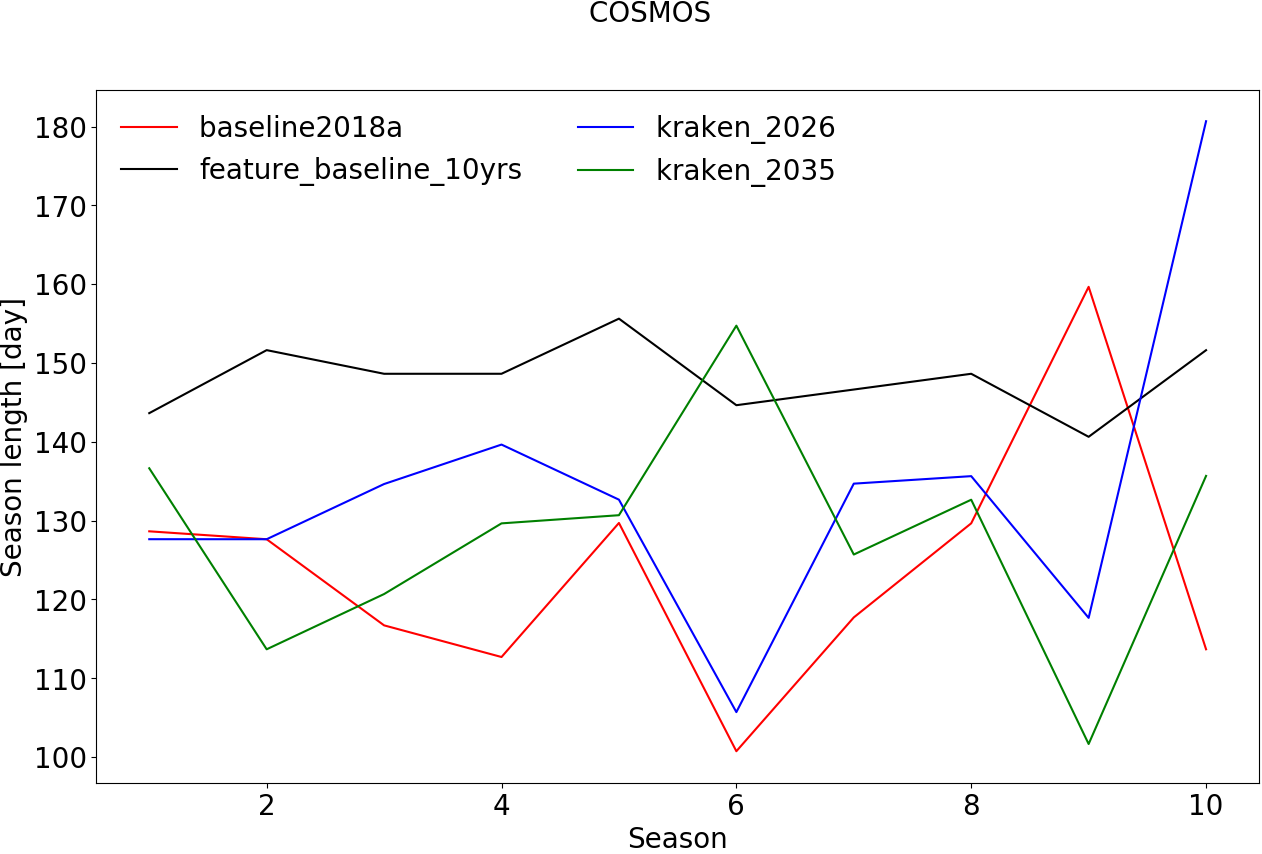
\includegraphics[width=10cm]{Figures/COSMOS_season_length.png}
  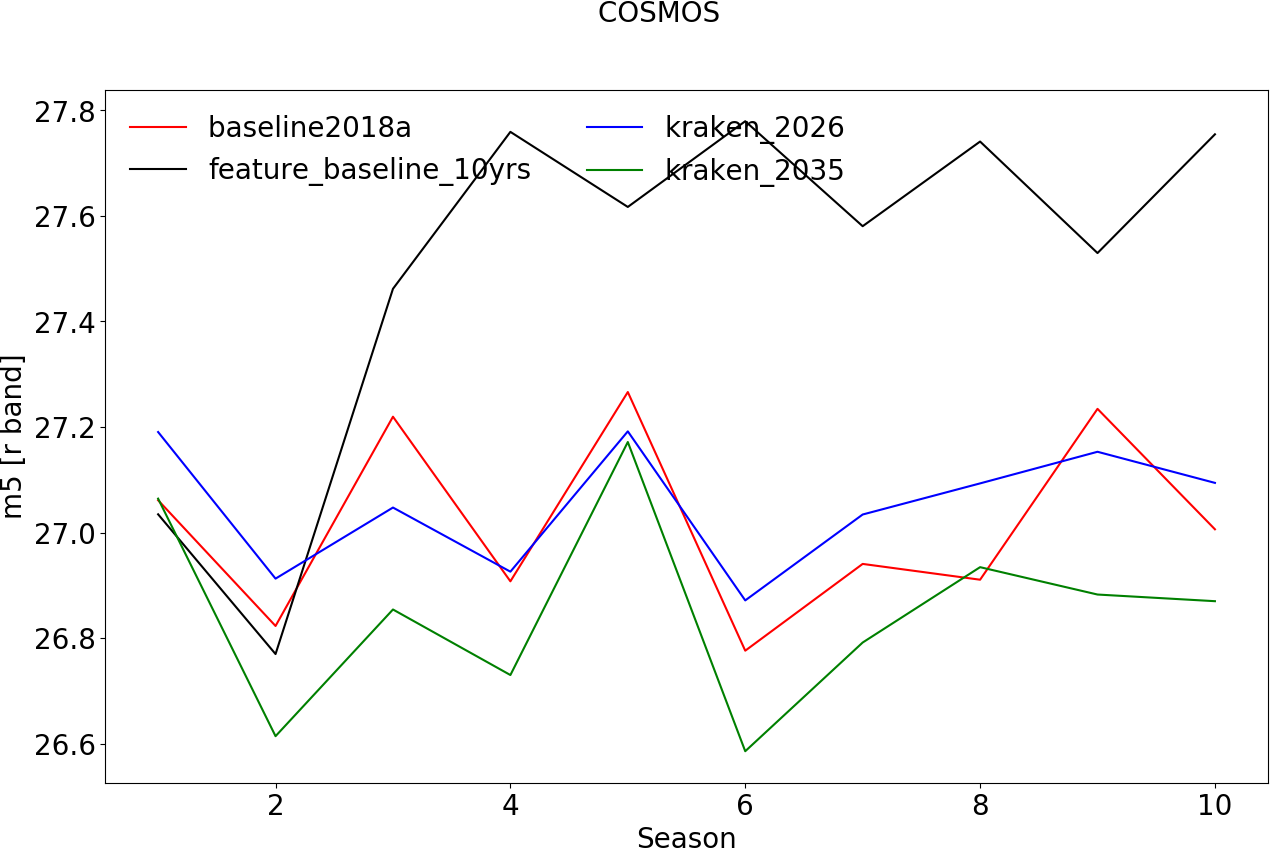
\includegraphics[width=10cm]{Figures/COSMOS_m5.png}
  %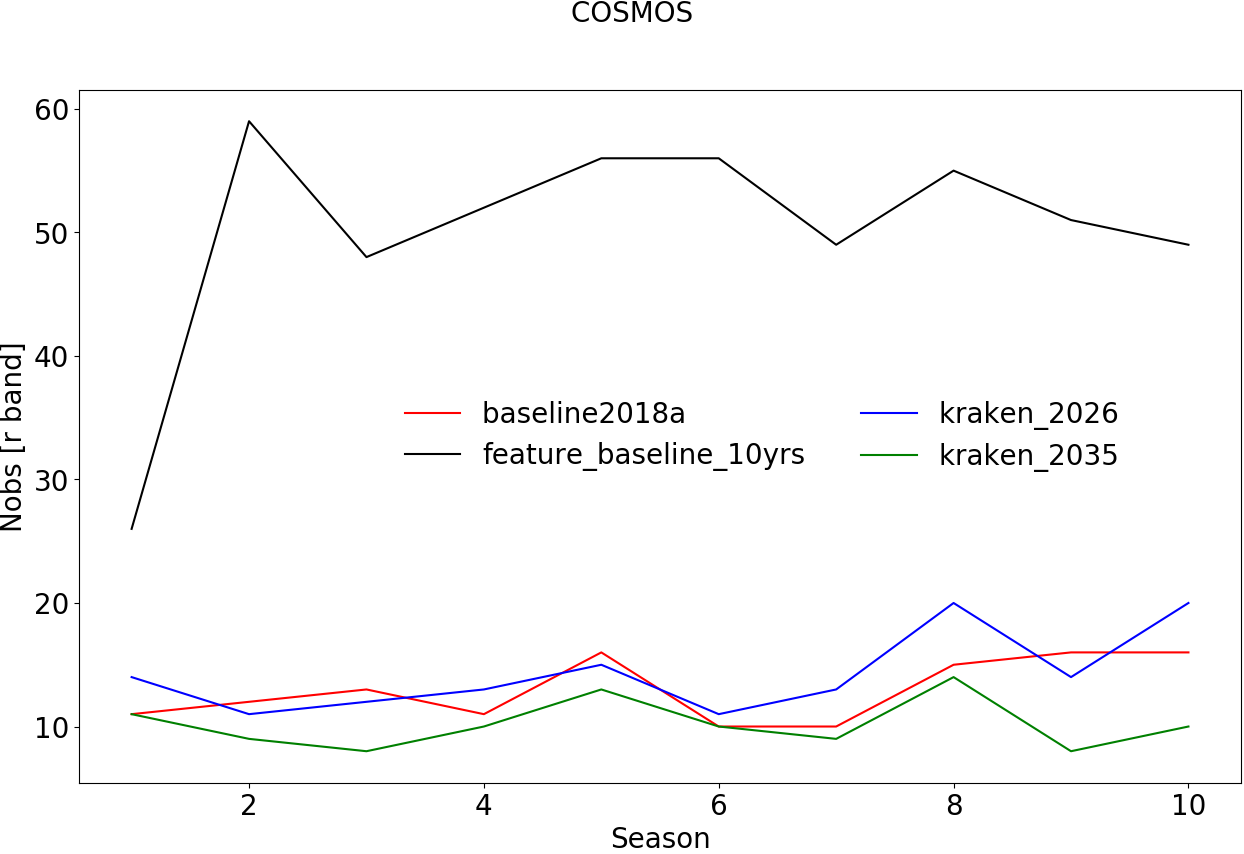
\includegraphics[width=10cm]{Figures/COSMOS_Nobs.png}
 \caption{Cadence (top, in day), season length (middle, in day) and coadded m5 (bottom, in mag) as a function of the season for the COSMOS field and baseline18a, feature\_baseline\_10yrs, kralen\_2026 and kraken\_2035 observing strategies.}\label{fig:cosmos_cad}
\end{center}
\end{figure}

\begin{figure}[htbp]
\begin{center}
  
  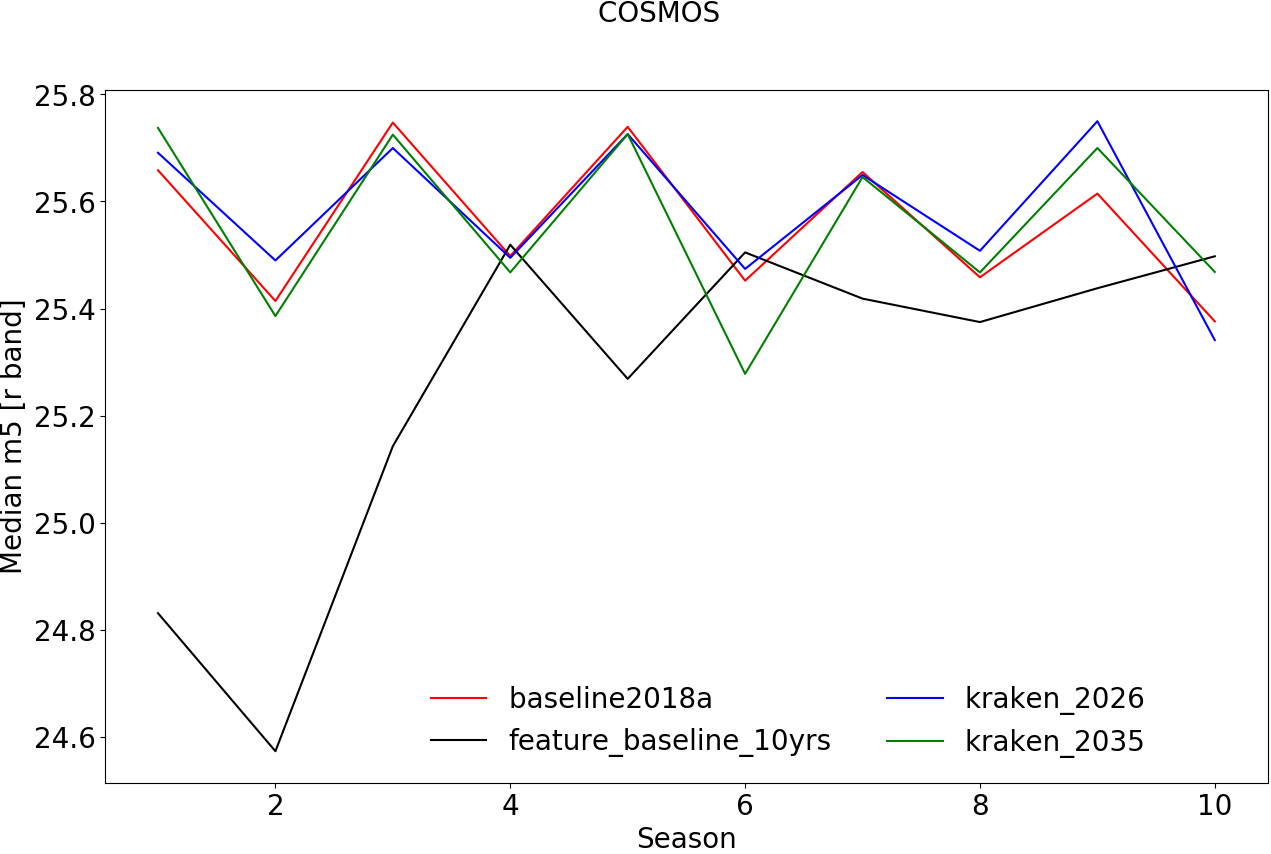
\includegraphics[width=10cm]{Figures/COSMOS_med_m5.png}
  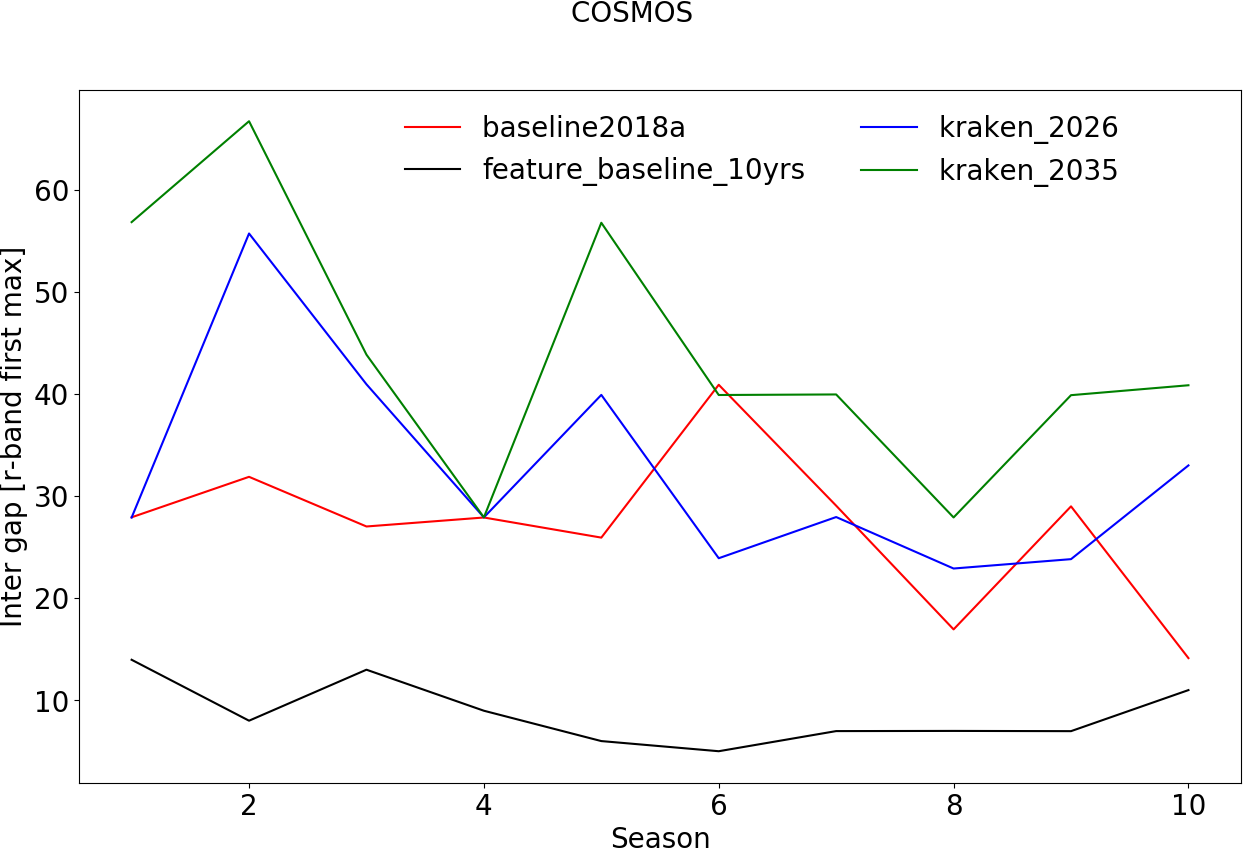
\includegraphics[width=10cm]{Figures/COSMOS_intergap_max1.png}
    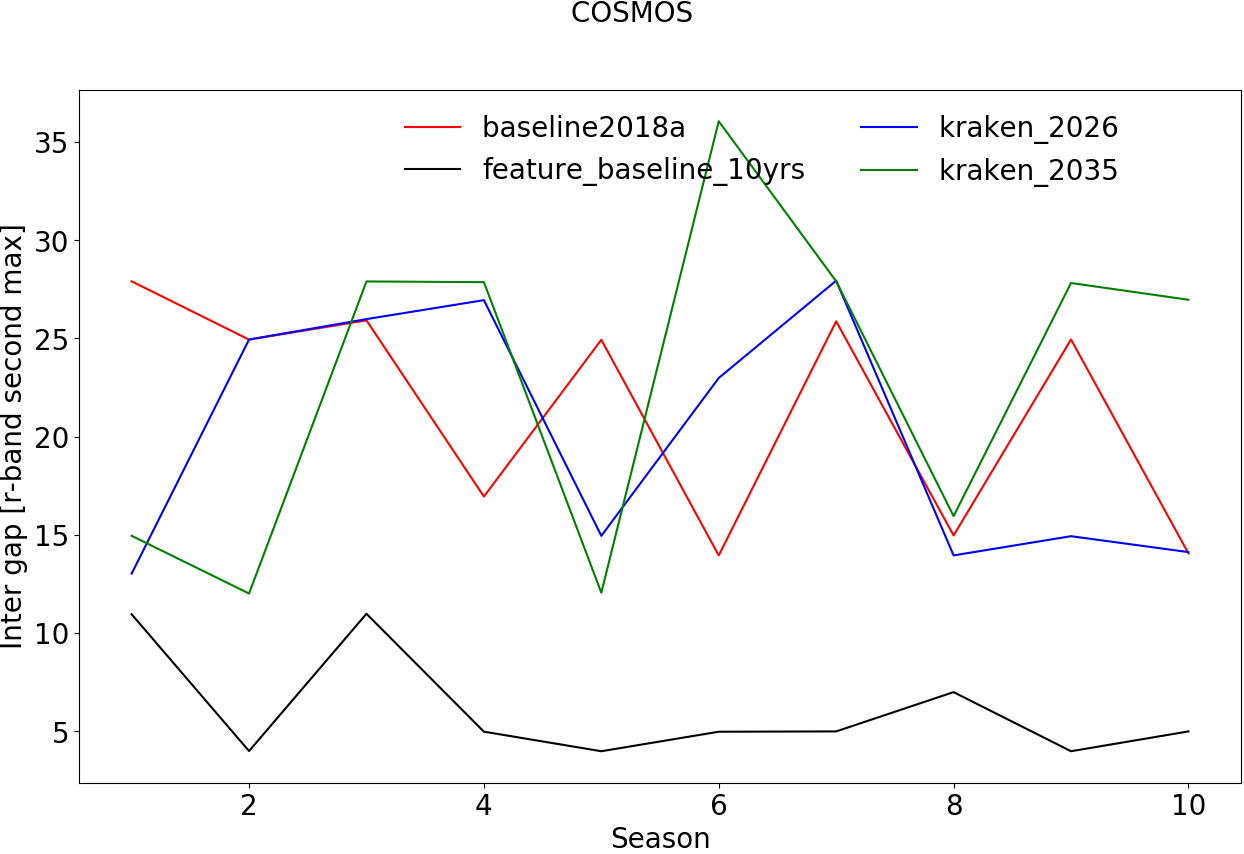
\includegraphics[width=10cm]{Figures/COSMOS_intergap_max2.png}
 \caption{Median m5 (top, in mag), first maximum inter-night gap (middle, in day) and second maximum inter-night gap (bottom, in day)  as a function of the season for the COSMOS field and baseline18a, feature\_baseline\_10yrs, kralen\_2026 and kraken\_2035 observing strategies.}\label{fig:cosmos_m5}
\end{center}
\end{figure}

%%%%%%%%%%%%%%%%%%%%%%%%%%%%%%%%%%%%%%%%%%%%%%


\begin{figure}[htbp]
\begin{center}
  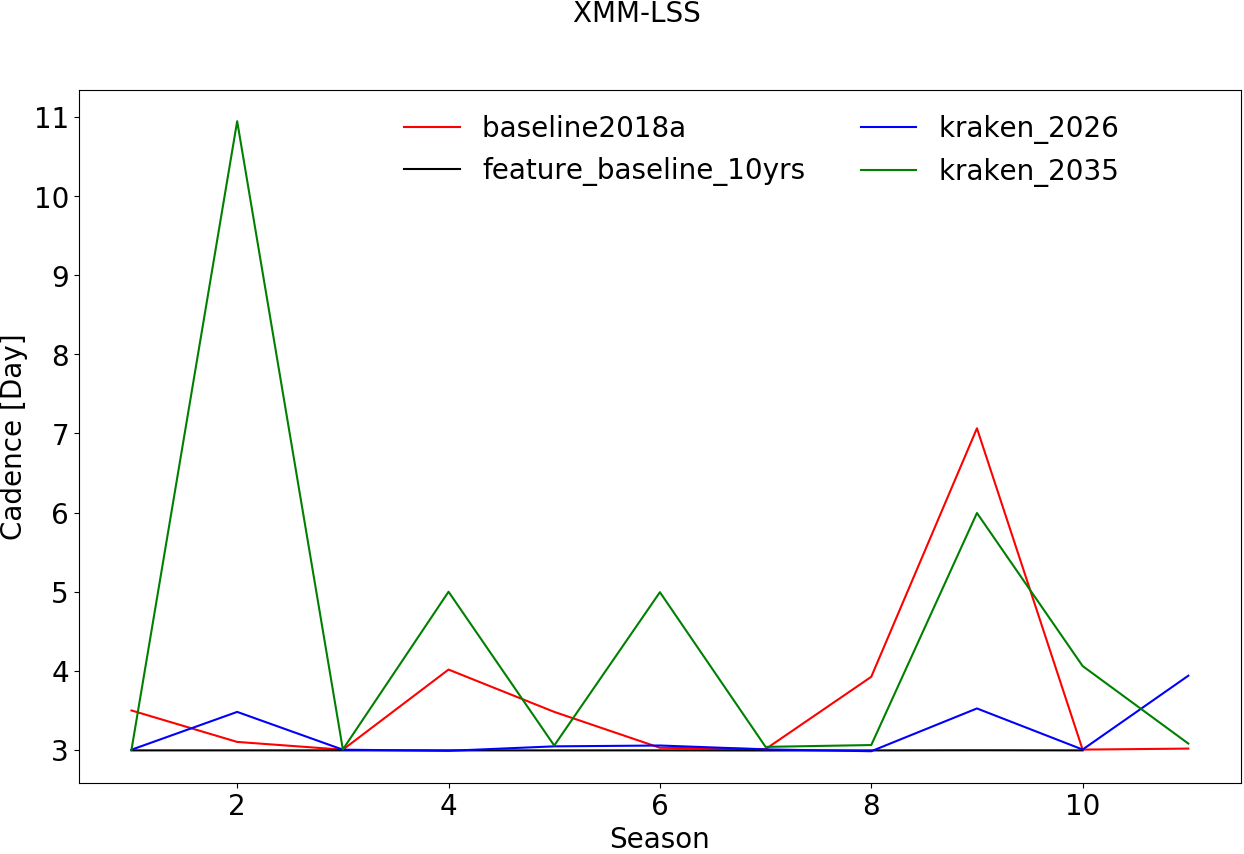
\includegraphics[width=10cm]{Figures/XMM-LSS_cadence.png}
  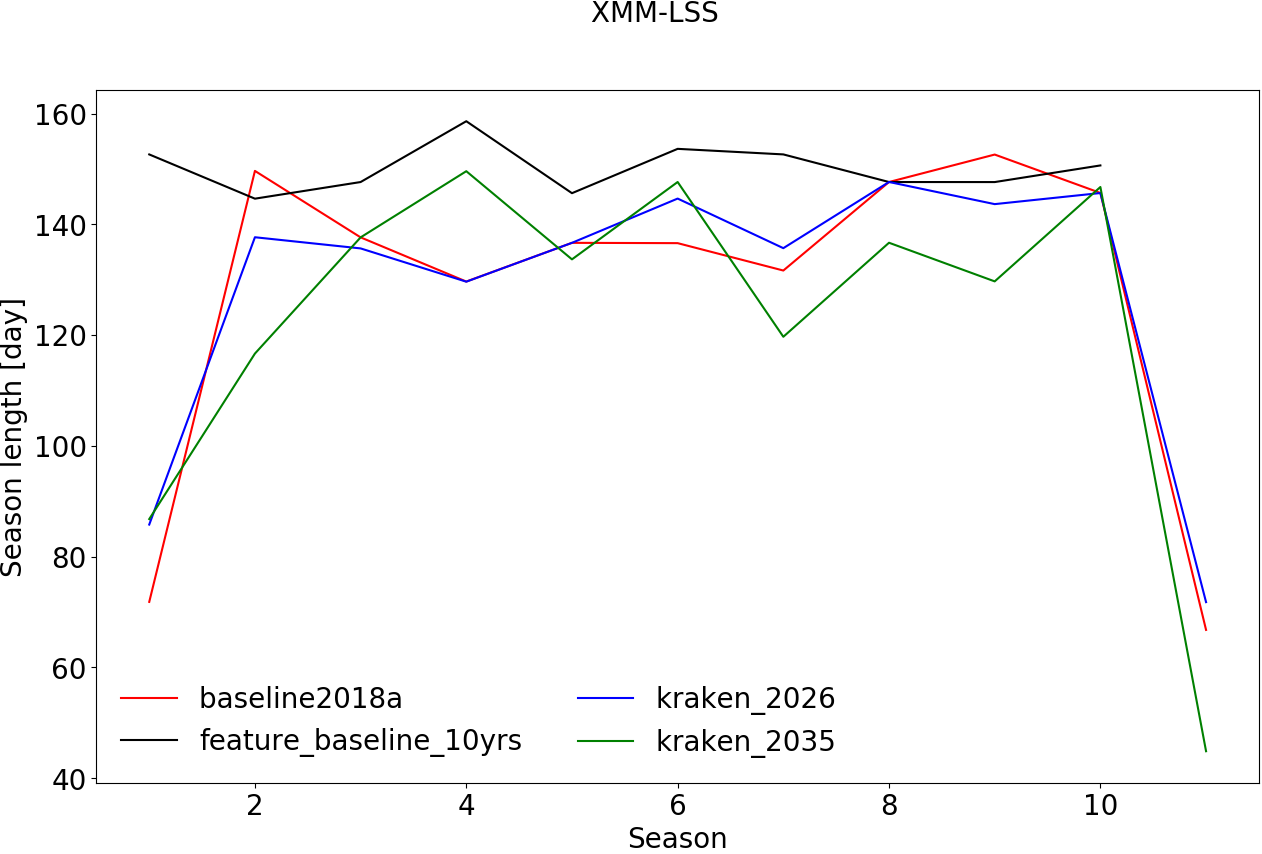
\includegraphics[width=10cm]{Figures/XMM-LSS_season_length.png}
  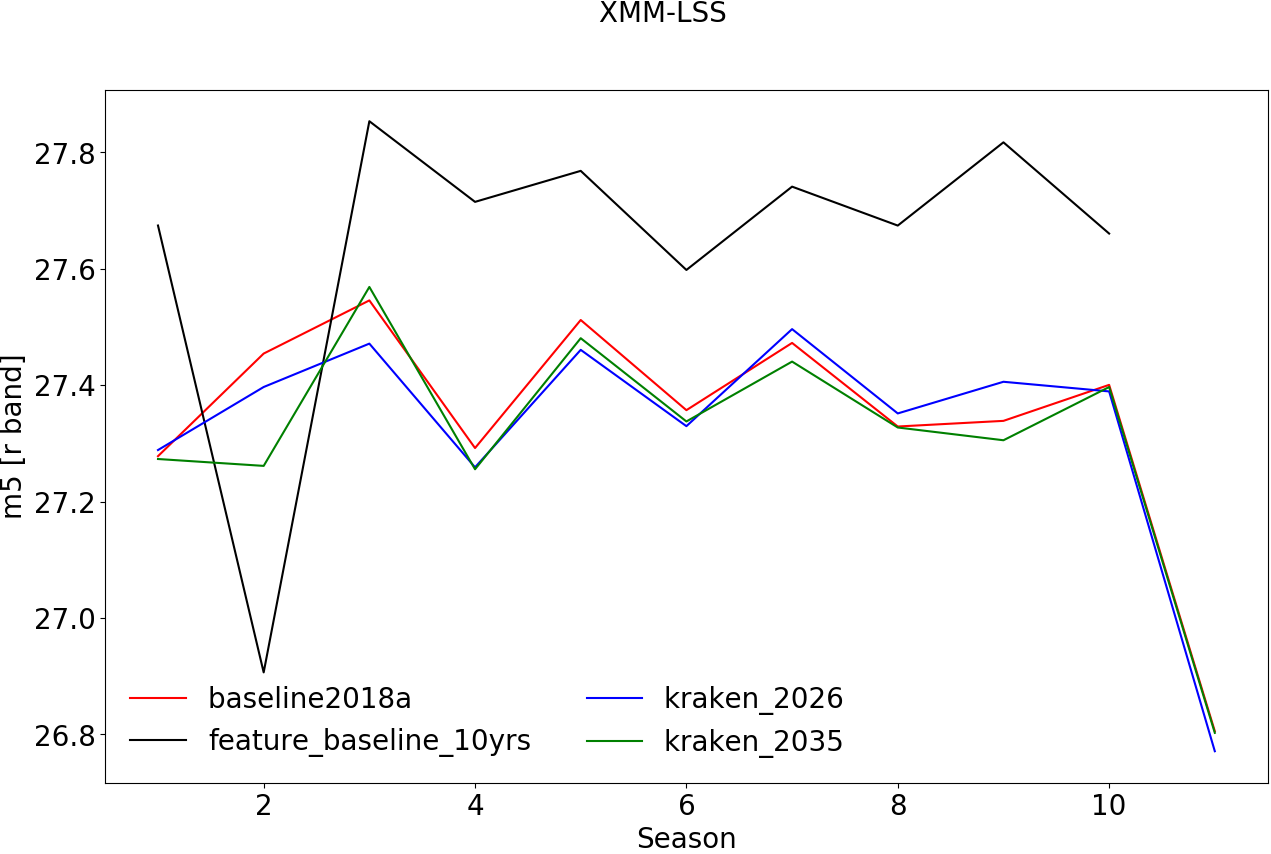
\includegraphics[width=10cm]{Figures/XMM-LSS_m5.png}
  %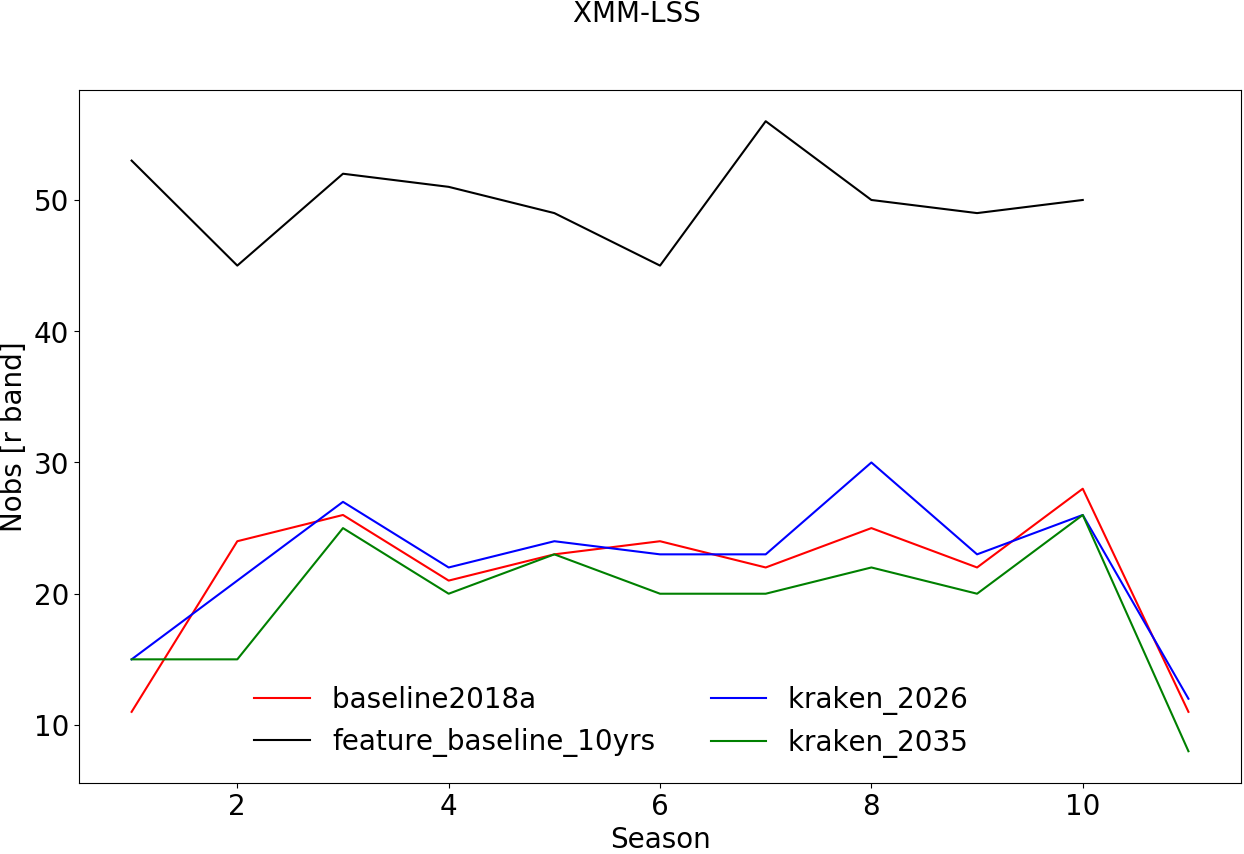
\includegraphics[width=10cm]{Figures/XMM-LSS_Nobs.png}
 \caption{Cadence (top, in day), season length (middle, in day) and coadded m5 (bottom, in mag) as a function of the season for the XMM-LSS field and baseline18a, feature\_baseline\_10yrs, kralen\_2026 and kraken\_2035 observing strategies.}\label{fig:xmm-lss_cad}
\end{center}
\end{figure}

\begin{figure}[htbp]
\begin{center}
  
  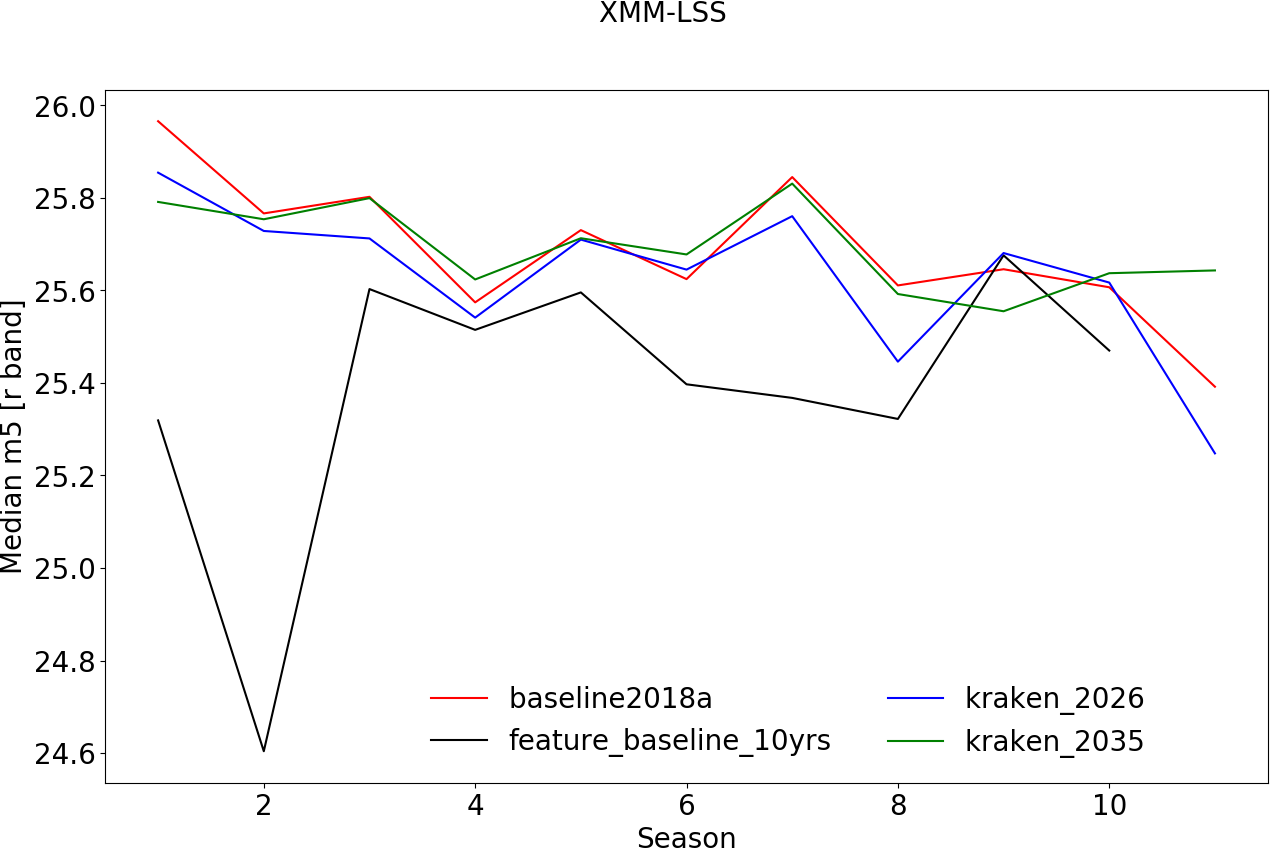
\includegraphics[width=10cm]{Figures/XMM-LSS_med_m5.png}
  \includegraphics[width=10cm]{Figures/XMM-LSS_intergap_max1.png}
    \includegraphics[width=10cm]{Figures/XMM-LSS_intergap_max2.png}
 \caption{Median m5 (top, in mag), first maximum inter-night gap (middle, in day) and second maximum inter-night gap (bottom, in day)  as a function of the season for the XMM-LSS field and baseline18a, feature\_baseline\_10yrs, kralen\_2026 and kraken\_2035 observing strategies.}\label{fig:xmm-lss_m5}
\end{center}
\end{figure}


%%%%%%%%%%%%%%%%%%%%%%%%%%%%%%%%%%%%%%%%%%%%%%


\begin{figure}[htbp]
\begin{center}
  \includegraphics[width=10cm]{Figures/CDFS_cadence.png}
  \includegraphics[width=10cm]{Figures/CDFS_season_length.png}
  \includegraphics[width=10cm]{Figures/CDFS_m5.png}
  %\includegraphics[width=10cm]{Figures/CDFS_Nobs.png}
 \caption{Cadence (top, in day), season length (middle, in day) and coadded m5 (bottom, in mag) as a function of the season for the CDFS field and baseline18a, feature\_baseline\_10yrs, kralen\_2026 and kraken\_2035 observing strategies.}\label{fig:cdfs_cad}
\end{center}
\end{figure}

\begin{figure}[htbp]
\begin{center}
  
  \includegraphics[width=10cm]{Figures/CDFS_med_m5.png}
  \includegraphics[width=10cm]{Figures/CDFS_intergap_max1.png}
    \includegraphics[width=10cm]{Figures/CDFS_intergap_max2.png}
 \caption{Median m5 (top, in mag), first maximum inter-night gap (middle, in day) and second maximum inter-night gap (bottom, in day)  as a function of the season for the CDFS field and baseline18a, feature\_baseline\_10yrs, kralen\_2026 and kraken\_2035 observing strategies.}\label{fig:cdfs_m5}
\end{center}
\end{figure}


%%%%%%%%%%%%%%%%%%%%%%%%%%%%%%%%%%%%%%%%%%%%%%


\begin{figure}[htbp]
\begin{center}
  \includegraphics[width=10cm]{Figures/ELAIS-S1_cadence.png}
  \includegraphics[width=10cm]{Figures/ELAIS-S1_season_length.png}
  \includegraphics[width=10cm]{Figures/ELAIS-S1_m5.png}
  %\includegraphics[width=10cm]{Figures/ELAIS-S1_Nobs.png}
 \caption{Cadence (top, in day), season length (middle, in day) and coadded m5 (bottom, in mag) as a function of the season for the ELAIS-S1 field and baseline18a, feature\_baseline\_10yrs, kralen\_2026 and kraken\_2035 observing strategies.}\label{fig:elais-s1_cad}
\end{center}
\end{figure}

\begin{figure}[htbp]
\begin{center}
  
  \includegraphics[width=10cm]{Figures/ELAIS-S1_med_m5.png}
  \includegraphics[width=10cm]{Figures/ELAIS-S1_intergap_max1.png}
    \includegraphics[width=10cm]{Figures/ELAIS-S1_intergap_max2.png}
 \caption{Median m5 (top, in mag), first maximum inter-night gap (middle, in day) and second maximum inter-night gap (bottom, in day)  as a function of the season for the ELAIS-S1 field and baseline18a, feature\_baseline\_10yrs, kralen\_2026 and kraken\_2035 observing strategies.}\label{fig:elais-s1_m5}
\end{center}
\end{figure}


%%%%%%%%%%%%%%%%%%%%%%%%%%%%%%%%%%%%%%%%%%%%%%


\begin{figure}[htbp]
\begin{center}
  \includegraphics[width=10cm]{Figures/SPT-DEEP_cadence.png}
  \includegraphics[width=10cm]{Figures/SPT-DEEP_season_length.png}
  \includegraphics[width=10cm]{Figures/SPT-DEEP_m5.png}
  %\includegraphics[width=10cm]{Figures/SPT DEEP_Nobs.png}
 \caption{Cadence (top, in day), season length (middle, in day) and coadded m5 (bottom, in mag) as a function of the season for the SPT DEEP field and baseline18a, feature\_baseline\_10yrs, kralen\_2026 and kraken\_2035 observing strategies.}\label{fig:spt deep_cad}
\end{center}
\end{figure}

\begin{figure}[htbp]
\begin{center}
  
  \includegraphics[width=10cm]{Figures/SPT-DEEP_med_m5.png}
  \includegraphics[width=10cm]{Figures/SPT-DEEP_intergap_max1.png}
    \includegraphics[width=10cm]{Figures/SPT-DEEP_intergap_max2.png}
 \caption{Median m5 (top, in mag), first maximum inter-night gap (middle, in day) and second maximum inter-night gap (bottom, in day)  as a function of the season for the SPT DEEP field and baseline18a, feature\_baseline\_10yrs, kralen\_2026 and kraken\_2035 observing strategies.}\label{fig:spt deep_m5}
\end{center}
\end{figure}


%%%%%%%%%%%%%%%%%%%%%%%%%%%%%%%%%%%%%%%%%%%%%%


\begin{figure}[htbp]
\begin{center}
  \includegraphics[width=10cm]{Figures/kraken_2035_cadence.png}
  \includegraphics[width=10cm]{Figures/kraken_2035_season_length.png}
  \includegraphics[width=10cm]{Figures/kraken_2035_m5.png}
  %\includegraphics[width=10cm]{Figures/SPT DEEP_Nobs.png}
 \caption{Cadence (top, in day), season length (middle, in day) and coadded m5 (bottom, in mag) as a function of the season for \ddfa, \ddfb, \ddfb and \ddfd fields and kraken\_2035 observing strategy.}\label{fig:kraken_cad}
\end{center}
\end{figure}

\begin{figure}[htbp]
\begin{center}
  
  \includegraphics[width=10cm]{Figures/kraken_2035_med_m5.png}
  \includegraphics[width=10cm]{Figures/kraken_2035_intergap_max1.png}
    \includegraphics[width=10cm]{Figures/kraken_2035_intergap_max2.png}
    \caption{Median m5 (top, in mag), first maximum inter-night gap (middle, in day) and second maximum inter-night gap (bottom, in day)  as a function of the season for \ddfa, \ddfb, \ddfb and \ddfd fields and kraken\_2035 observing strategy.}\label{fig:kraken_m5}
\end{center}
\end{figure}


\clearpage

\section{Cadence metric: a simple metric for SN that may be implemented in OpSim/SLAIR}
\label{sec:cadencemetric}

If we fit a light curve model $L(t) = A \times \ell(t)$ on a
lightcurve $(t_i, y_i, \sigma_i)$, the least square estimate of $A$ is
given by:
$$
\hat{A} = \frac{\sum w_i \ell_i y_i}{\sum w_i \ell_i^2}
$$
and the signal-to-noise ratio on $\hat{A}$ is:
$$
SNR = \sum_i (w_i L_i^2)^{1/2}
$$ since we are in the background dominated regime, the weights may be
expressed as a function of the $5-\sigma$ limiting flux of each visit
$f_{i|5}$, and we have:
$$
SNR_{\mathrm{band}} = \sum_{i} 5 \times (f^{-2}_{i|5} L_i^2)^{1/2}
$$
where $5-\sigma$ limiting flux of each visit $f_{i|5}$.

This metrics is simple in the sense that it does not require to use a SN
light curve fitter. One just need lightcurve templates and the
limiting magnitudes of each visit -- given in the cadence
databases. In practice, using $SNR_g > 30, SNR_r > 40, SNR_i > 30$
(for $z<0.3$), and $SNR_r > 40$, $SNR_i > 30$ and $SNR_z > 20$ for
$z>0.3$ allows to fulfill the requirement on color resolution above.

\clearpage

\section{Overlap with 4MOST}

  \begin{figure}[!htbp]
    \caption{Left: the LSST Healpix maps colour-coded by number of
    visits. Right: The corresponding 4MOST overlap map,
    where red represents the overlap area, blue represents areas of
    LSST WFD that have no 4MOST coverage and yellow represents 4MOST
    area with no LSST coverage. Note that the LSST DDFs are
    deliberately missing from the LSST maps in this analysis. }
    \label{overlap_maps}
    \begin{center}
  \begin{tabular}{cc}
    
    \includegraphics[width=7.0cm]{overlap_4MOST/colossus_2664_wfd_avail_ldep.png} & \includegraphics[width=7.0cm]{overlap_4MOST/colossus_2664_wfd_avail_overlap.png} \cr
    \includegraphics[width=7.0cm]{overlap_4MOST/colossus_2665_wfd_avail_ldep.png} & \includegraphics[width=7.0cm]{overlap_4MOST/colossus_2665_wfd_avail_overlap.png} \cr
    \includegraphics[width=7.0cm]{overlap_4MOST/colossus_2667_wfd_avail_ldep.png} & \includegraphics[width=7.0cm]{overlap_4MOST/colossus_2667_wfd_avail_overlap.png} \cr

  \end{tabular}
  \end{center}
\end{figure}

  %\begin{comment}
\begin{figure}[!htbp]
      \caption{continued}
      \label{overlap_maps_d}
   \begin{center}
  \begin{tabular}{cc}

    \includegraphics[width=7.0cm]{overlap_4MOST/kraken_2026_wfd_avail_ldep.png} & \includegraphics[width=7.0cm]{overlap_4MOST/kraken_2026_wfd_avail_overlap.png} \cr
    \includegraphics[width=7.0cm]{overlap_4MOST/kraken_2036_wfd_avail_ldep.png} & \includegraphics[width=7.0cm]{overlap_4MOST/kraken_2036_wfd_avail_overlap.png} \cr
    \includegraphics[width=7.0cm]{overlap_4MOST/mothra_2045_wfd_avail_ldep.png} & \includegraphics[width=7.0cm]{overlap_4MOST/mothra_2045_wfd_avail_overlap.png} \cr

  \end{tabular}
\end{center}
\end{figure}
%\end{comment}

\begin{figure}[!htbp]
\caption{continued}
\label{overlap_maps_c}
\begin{center}
  \begin{tabular}{cc}
    
    \includegraphics[width=7.0cm]{overlap_4MOST/pontus_2002_wfd_avail_ldep.png} & \includegraphics[width=7.0cm]{overlap_4MOST/pontus_2002_wfd_avail_overlap.png} \cr
    \includegraphics[width=7.0cm]{overlap_4MOST/pontus_2489_wfd_avail_ldep.png} & \includegraphics[width=7.0cm]{overlap_4MOST/pontus_2489_wfd_avail_overlap.png} \cr
    \includegraphics[width=7.0cm]{overlap_4MOST/pontus_2502_wfd_avail_ldep.png} & \includegraphics[width=7.0cm]{overlap_4MOST/pontus_2502_wfd_avail_overlap.png} \cr
        
  \end{tabular}
\end{center}
\end{figure}

%\end{comment}

\end{appendices}
